\documentclass[11pt,aspectratio=169]{beamer}
\usetheme{Warsaw}
\usepackage{fontspec}
\setmainfont[Ligatures=TeX]{Arial}
\usepackage{amsmath}
\usepackage{diagbox}
\usepackage[english]{babel}
\usepackage{graphicx}
\usepackage{varwidth}
\graphicspath{ {images/} }
\usepackage{tikz}

\usebackgroundtemplate{%
\tikz\node[opacity=0.2,inner sep=0] {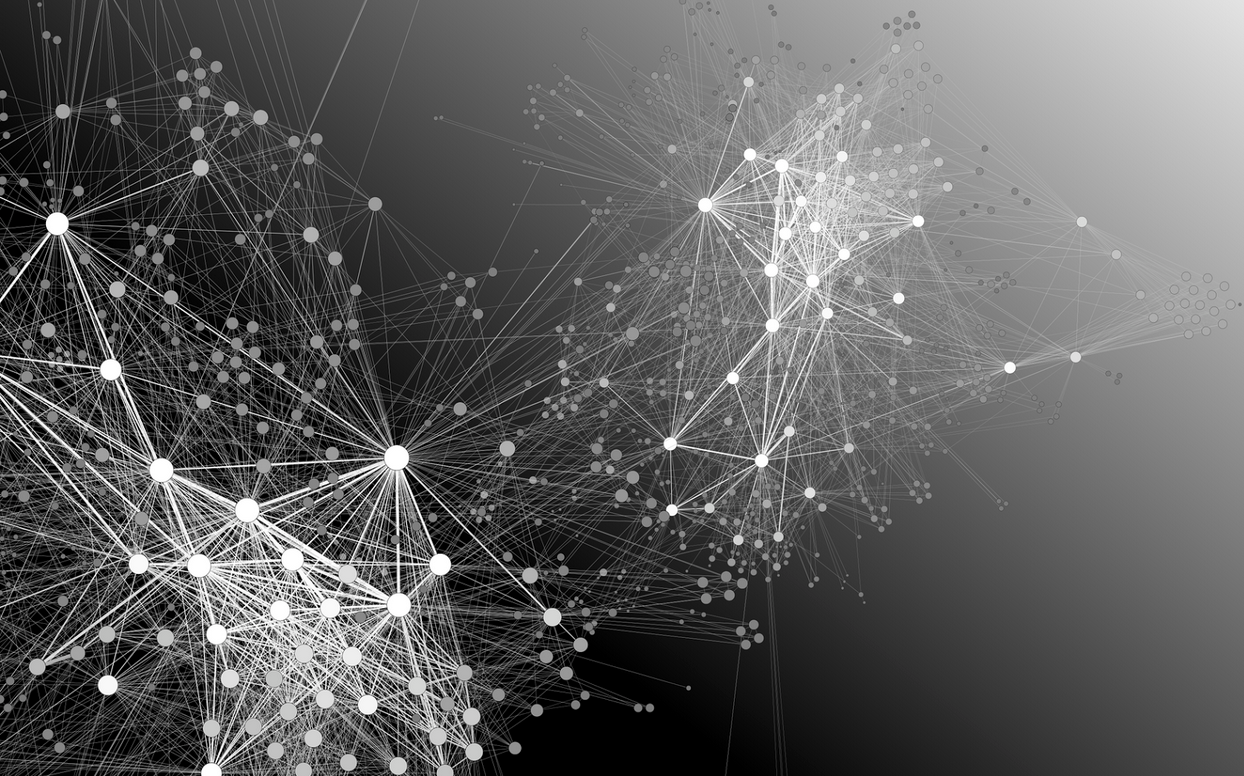
\includegraphics[height=\paperheight,width=\paperwidth]{background.png}};}
\setbeamertemplate{title page}[default][colsep=-4bp,rounded=true,shadow=false]
\AtBeginDocument{
    \pgfdeclareverticalshading{beamer@topshade}{0}{%
        color(0pt)=(black);
        color(4pt)=(black!50!bg)
    }
}

\title[Recursive Nearest Neighbors Methods in Recommender Systems \hspace{8mm}\insertframenumber/\inserttotalframenumber]{Recursive Nearest Neighbors Methods in Recommender Systems}
\author[Stylianos Tsesmetzis]{Stylianos Tsesmetzis\\{\small Supervisor: Nicholas Ampazis}}
\institute
{

\includegraphics[height=1cm,width=1cm]{cover.png}\\
 University of the Aegean\\
 School of Engineering\\
  Department of Financial and Management Engineering
}\date{October 31, 2017}

\subject{Recommender Systems}

\AtBeginSection
{\begin{frame}{Table of Contents}
\vspace{-1cm}
\tableofcontents[currentsection,hideothersubsections]
\end{frame}}

\begin{document}
%------------------------------------------------------------------Title------------------------------------------------------------------------------------------------------------
\begin{frame}
\titlepage
\end{frame}
\addtobeamertemplate{frametitle}{}{%
\begin{tikzpicture}[remember picture,overlay]
\node[anchor=north east,yshift=-40pt] at (current page.north east) {
\includegraphics[height=0.6cm]{cover.png}};
\end{tikzpicture}}
%-------------------------------------------------------------------ToC-------------------------------------------------------------------------------------------------------------
\begin{frame}
\frametitle{Table of Contents}
\vspace{-1cm}
\tableofcontents[hideallsubsections]
\end{frame}
%---------------------------------------------------------------Introduction--------------------------------------------------------------------------------------------------------
% !TeX root = ../main.tex

\section{Introduction}
\subsection{Recommender Systems Overview}
\begin{frame}[t]
    \frametitle{Recommender Systems Overview}
    \vspace{-1cm}
    \begin{itemize}
        \item<1->What is a recommender system and what does it do?\\
        \only<1-6>{
            \begin{enumerate}
                \item<2-> Predict how much a user may like a certain item
                \item<3-> Compose a list of N best items for a user
                \item<4-> Compose a list of N best users for a specific item
                \item<5-> Explain to the users why these items are recommended them
                \item<6-> Adjust the prediction and recommendation based on user's and
                other people feedback
            \end{enumerate}
        }
        \item<7->Why we need a recommender system?
        \only<7>{
            \begin{figure}
                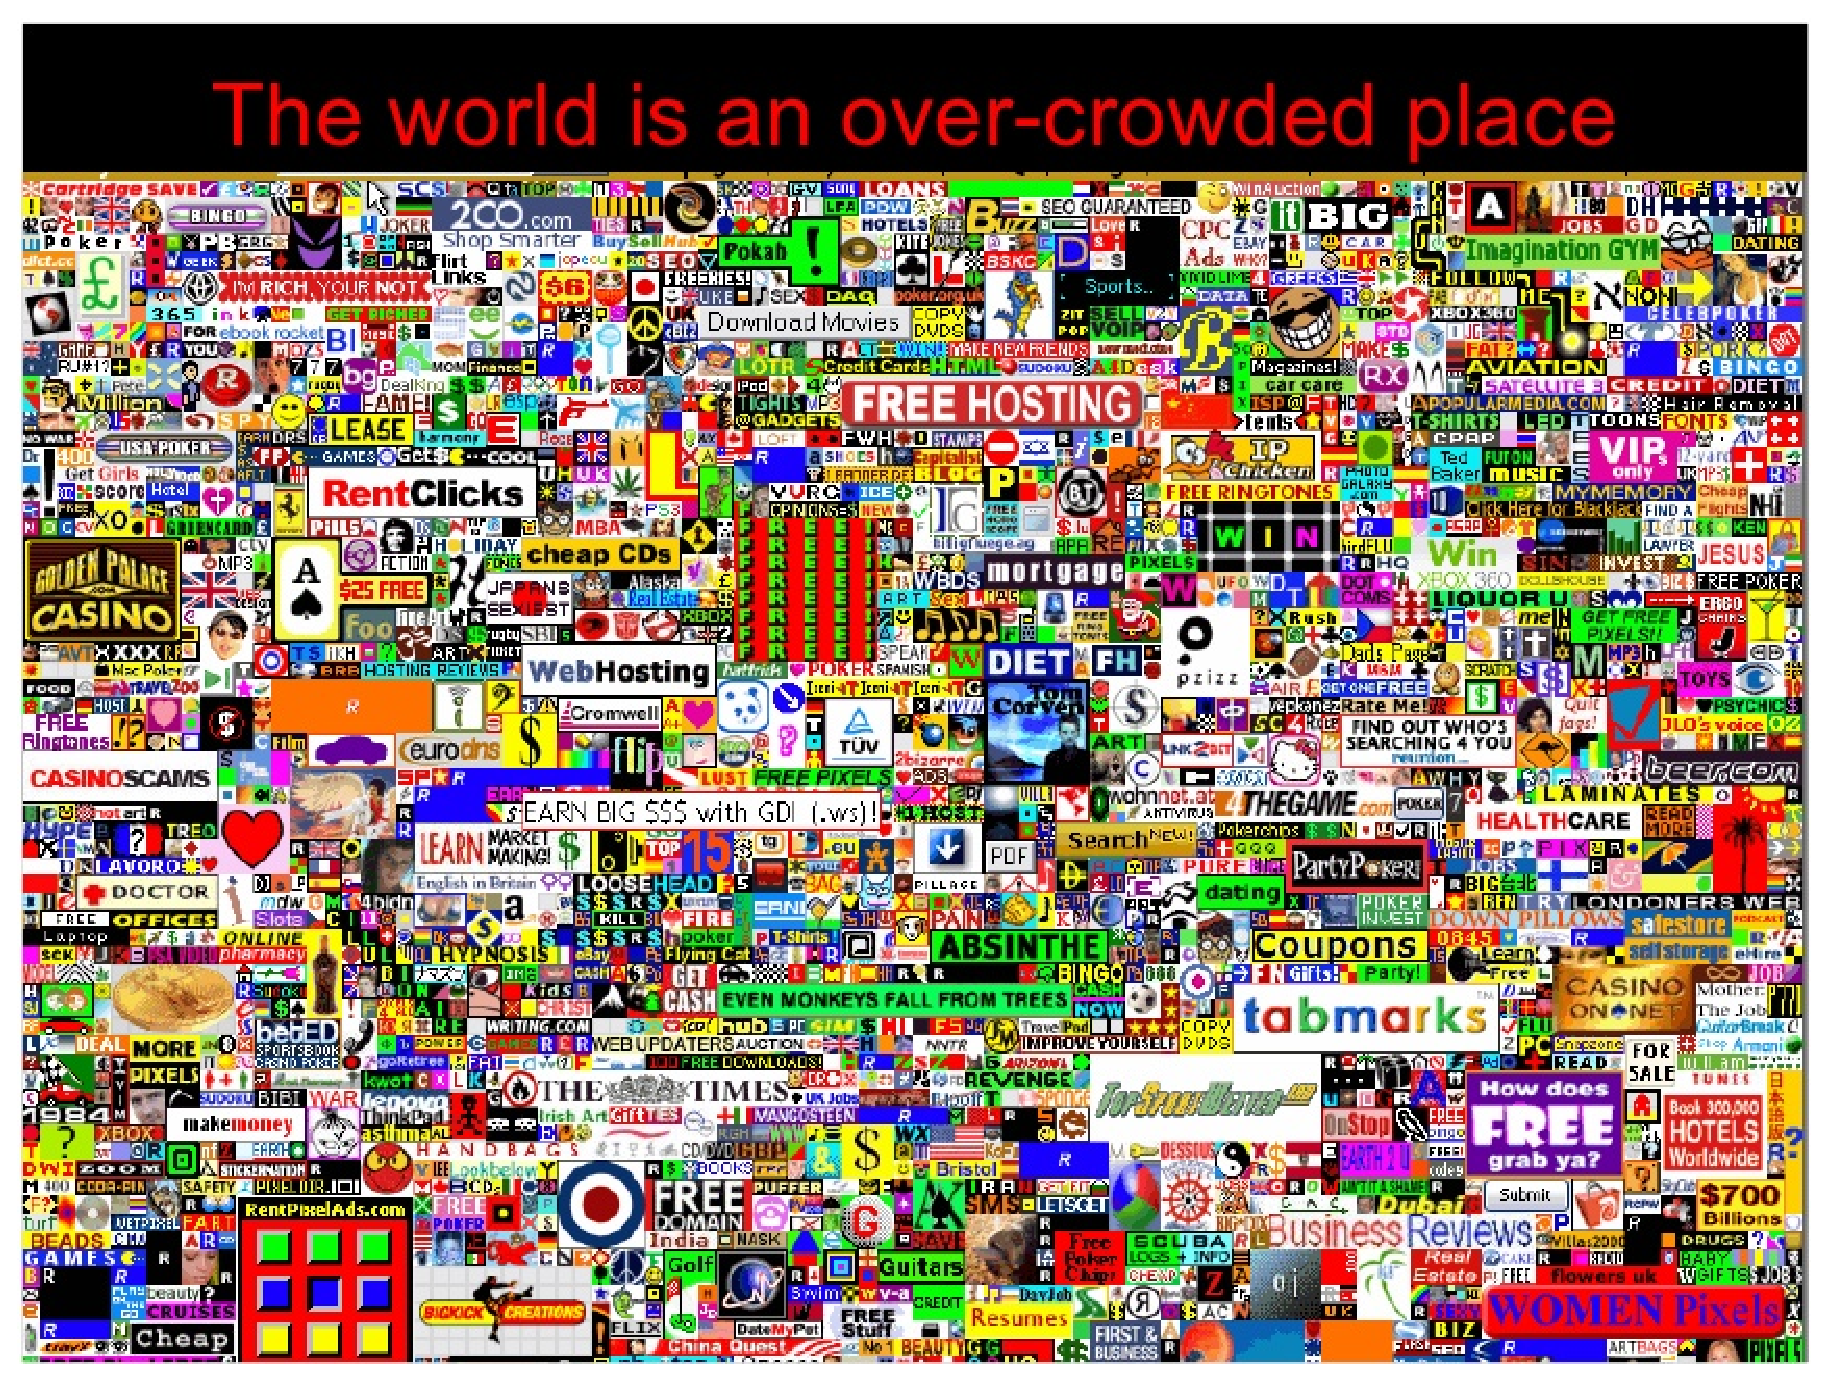
\includegraphics[width=0.7\textwidth,height=0.65\textheight]{overcrowded.eps}
            \end{figure}
        }
        \item<8->How we build a recommender system?
        \only<8-12>{
            \begin{enumerate}
                \item<9->\textbf{Collaborative Filtering}
                    \begin{itemize}
                        \item Neighborhood-based
                        \item Model-based
                    \end{itemize}
                \item<10->\textbf{Content-based}
                \item<11->\textbf{Knowledge Based}
                \item<12->\textbf{Hybrid}
            \end{enumerate}
        }
    \end{itemize}
\end{frame}
\subsection{Motivation}
\begin{frame}[t]
    \frametitle{Motivation}
    \centering
    \underline{\textbf{Problems with collaborative filtering}}
    \vspace{0.5cm}
    \begin{enumerate}
        \item \textbf{Scale}
        \begin{itemize}
            \item New users and items enter a recommendation platform everyday.
        \end{itemize}
        \item \textbf{Sparse data}
        \begin{itemize}
            \item A user has rated only one item or an item has been rated only once.
        \end{itemize}
        \item \textbf{Cold-Start}
        \begin{itemize}
            \item New users and items have no history.
        \end{itemize}
   \end{enumerate}
\end{frame}
\subsection{Approach}
\begin{frame}[t]
    \frametitle{Approach}
    \centering
    \underline{\textbf{Objectives}}
    \vspace{1cm}
    \begin{enumerate}
        \item Explain the Neighborhood-based Collaborative Filtering
        \item Propose the Recursive Nearest Neighbors Algorithm
        \item Present the Experimental results on the Epinions data set.
    \end{enumerate}
\end{frame}

%-----------------------------------------------------------Neighborhood-based CF---------------------------------------------------------------------------------------------------
% !TeX root = ../main.tex

\section{Neighborhood-based Collaborative Filtering}
\subsection{Introduction}
\begin{frame}
    \frametitle{Introduction}
    \centering
    \underline{\textbf{Collaborative Filtering}}
    \begin{itemize}
        \item \textbf{User-based}
            \begin{itemize}
                \item Many People like "The Godfather" should I watch it too?
                \item Choose a number of users who like things I like and
                      decide based on how much they liked it
                \item If we used to like similar items in the past, we will continue to like similar items in the future
            \end{itemize}
        \item \textbf{Item-based}
            \begin{itemize}
                \item Is "Jurassic Park" a good choice based on movies I usually see?
                \item Choose a number of movies that I have seen and share similar audience with "Jurassic Park",
                then decide based on how much I liked the previous movies
                \item If I liked these type of items in the past, I will probably also like those items
            \end{itemize}
    \end{itemize}
\end{frame}
\begin{frame}[t]
    \frametitle{Introduction}
    \centering
    \underline{\textbf{Advantages of Collaborative Filtering}}
    \begin{center}
        \begin{enumerate}
            \item Simplicity
            \item Justifiability
            \item Efficiency
            \item Stability
        \end{enumerate}
    \end{center}
\end{frame}

\subsection{Similarity Function Variants}
\begin{frame}
    \frametitle{Cosine Similarity}
    \begin{columns}
        \column{0.5\textwidth}
        \centering
        \underline{\textbf{User-based}}
        \begin{equation*}
            cos(u,v) = \frac{\sum_{i \in \mathcal{I}_{uv}}r_{ui}r_{vi}}
        		    {\sqrt{\sum_{i \in \mathcal{I}_{u}}r_{ui}^2}
        		     \sqrt{\sum_{i \in \mathcal{I}_{v}}r_{vi}^2}}
        \end{equation*}
        \tiny
        \begin{itemize}
            \item $\mathcal{I}_{u}:$ The set of items that have been rated by user $u$
            \item $\mathcal{I}_{v}:$ The set of items that have been rated by user $v$
            \item $\mathcal{I}_{uv}:$ The set of items that users $u$ and $v$ rated in common
            \item $r_{ui}:$ The rating that user $u$ gave to item $i$
            \item $r_{vi}:$ The rating that user $v$ gave to item $i$
        \end{itemize}
        \column{0.5\textwidth}
        \centering
        \underline{\textbf{Item-based}}
        \begin{equation*}
            cos(i,j) = \frac{\sum_{u \in \mathcal{U}_{ij}}r_{iu}r_{ju}}
        		    {\sqrt{\sum_{u \in \mathcal{U}_{i}}r_{iu}^2}
        		     \sqrt{\sum_{u \in \mathcal{U}_{j}}r_{ju}^2}}
        \end{equation*}
        \tiny
        \begin{itemize}
            \item $\mathcal{U}_{i}:$ The set of users that have rated item $i$
            \item $\mathcal{U}_{j}:$ The set of users that have rated item $j$
            \item $\mathcal{U}_{ij}:$ The set of users that have both rated items $i$ and $j$
            \item $r_{iu}:$ The rating item $i$ received from user $u$
            \item $r_{ju}:$ The rating item $j$ received from user $u$
        \end{itemize}
    \end{columns}
\end{frame}
\begin{frame}
    \frametitle{Modified Cosine Similarity}
    \begin{columns}
        \column{0.5\textwidth}
        \centering
        \underline{\textbf{User-based}}
        \begin{equation*}
            MC(u,v) = \frac{\sum_{i \in \mathcal{I}_{uv}}r_{ui}r_{vi}}
		   {\sqrt{\sum_{i \in \mathcal{I}_{uv}}r_{ui}^2}
                    \sqrt{\sum_{i \in \mathcal{I}_{uv}}r_{vi}^2}}
        \end{equation*}
        \tiny
        \begin{itemize}
            \item $\mathcal{I}_{uv}:$ The set of items that users $u$ and $v$ rated in common
            \item $r_{ui}:$ The rating that user $u$ gave to item $i$
            \item $r_{vi}:$ The rating that user $v$ gave to item $i$
        \end{itemize}
        \column{0.5\textwidth}
        \centering
        \underline{\textbf{Item-based}}
        \begin{equation*}
            MC(i,j) = \frac{\sum_{u \in \mathcal{U}_{ij}}r_{iu}r_{ju}}
		   {\sqrt{\sum_{u \in \mathcal{U}_{ij}}r_{iu}^2}
                    \sqrt{\sum_{u \in \mathcal{U}_{ij}}r_{ju}^2}}
        \end{equation*}
        \tiny
        \begin{itemize}
            \item $\mathcal{U}_{ij}:$ The set of users that have both rated items $i$ and $j$
            \item $r_{iu}:$ The rating item $i$ received from user $u$
            \item $r_{ju}:$ The rating item $j$ received from user $u$
        \end{itemize}
    \end{columns}
\end{frame}
\begin{frame}
    \frametitle{Adjusted Cosine Similarity}
    \vspace{-0.8cm}
    \begin{columns}
        \column{0.5\textwidth}
        \centering
        \underline{\textbf{User-based}}
        \begin{equation*}
            \small
            \begin{split}
            &AC(u,v) = \frac{\sum_{i \in \mathcal{I}_{uv}}(r_{ui}-\bar{r_{i}})(r_{vi}-\bar{r_{i}})}
        		    {\sqrt{\sum_{i \in \mathcal{I}_{uv}}(r_{ui}-\bar{r_{i}})^2}
                             \sqrt{\sum_{i \in \mathcal{I}_{uv}}(r_{vi}-\bar{r_{i}})^2}} \\\\
            &\bar{r_{i}} = \frac{\sum_{u \in \mathcal{U}_i}r_{iu}}
         		        {\mathopen|\mathcal{U}_i\mathclose|}
            \end{split}
        \end{equation*}
        \tiny
        \begin{itemize}
            \item $\mathcal{I}_{uv}:$ The set of items that users $u$ and $v$ rated in common
            \item $r_{ui}:$ The rating that user $u$ gave to item $i$
            \item $r_{vi}:$ The rating that user $v$ gave to item $i$
            \item $\mathcal{U}_{i}:$ The set of users that have rated item $i$
            \item $\bar{r_{i}}:$ The mean rating of item $i$

        \end{itemize}
        \column{0.5\textwidth}
        \centering
        \underline{\textbf{Item-based}}
        \begin{equation*}
            \small
            \begin{split}
            &AC(i,j) = \frac{\sum_{u \in \mathcal{U}_{ij}}(r_{iu}-\bar{r_{u}})(r_{ju}-\bar{r_{u}})}
        		    {\sqrt{\sum_{u \in \mathcal{U}_{ij}}(r_{iu}-\bar{r_{u}})^2}
                             \sqrt{\sum_{u \in \mathcal{U}_{ij}}(r_{ju}-\bar{r_{u}})^2}} \\\\
            &\bar{r_{u}} = \frac{\sum_{i \in \mathcal{I}_u}r_{ui}}
         		        {\mathopen|\mathcal{I}_u\mathclose|}
            \end{split}
        \end{equation*}
        \tiny
        \begin{itemize}
            \item $\mathcal{U}_{ij}:$ The set of users that have both rated items $i$ and $j$
            \item $r_{iu}:$ The rating item $i$ received from user $u$
            \item $r_{ju}:$ The rating item $j$ received from user $u$
            \item $\mathcal{I}_{u}:$ The set of items that have been rated by user $u$
            \item $\bar{r_{u}}:$ The mean rating of user $u$
        \end{itemize}
    \end{columns}
\end{frame}
\begin{frame}
    \frametitle{Modified Adjusted Cosine Similarity}
    \vspace{-0.6cm}
    \begin{columns}
        \column{0.5\textwidth}
        \centering
        \underline{\textbf{User-based}}
        \begin{equation*}
        \footnotesize
        \begin{split}
        &MAC(u,v) = \frac{\sum_{i \in \mathcal{I}_{uv}}(r_{ui}-\bar{r_{i}})(r_{vi}-\bar{r_{i}})}
                         {\sqrt{\sum_{i \in \mathcal{I}_{u}}(r_{ui}-\bar{r_{i}})^2}
                          \sqrt{\sum_{i \in \mathcal{I}_{v}}(r_{vi}-\bar{r_{i}})^2}} \\\\
        &\bar{r_{i}} = \frac{\sum_{u \in \mathcal{U}_i}r_{iu}}
                            {\mathopen|\mathcal{U}_i\mathclose|}
        \end{split}
        \end{equation*}
        \tiny
        \begin{itemize}
            \item $\mathcal{I}_{u}:$ The set of items that have been rated by user $u$
            \item $\mathcal{I}_{v}:$ The set of items that have been rated by user $v$
            \item $\mathcal{I}_{uv}:$ The set of items that users $u$ and $v$ rated in common
            \item $r_{ui}:$ The rating that user $u$ gave to item $i$
            \item $r_{vi}:$ The rating that user $v$ gave to item $i$
            \item $\mathcal{U}_{i}:$ The set of users that have rated item $i$
            \item $\bar{r_{i}}:$ The mean rating of item $i$
        \end{itemize}
        \column{0.5\textwidth}
        \centering
        \underline{\textbf{Item-based}}
        \begin{equation*}
        \footnotesize
        \begin{split}
        &MAC(i,j) = \frac{\sum_{u \in \mathcal{U}_{ij}}(r_{iu}-\bar{r_{u}})(r_{ju}-\bar{r_{u}})}
                         {\sqrt{\sum_{u \in \mathcal{U}_{i}}(r_{iu}-\bar{r_{u}})^2}
                          \sqrt{\sum_{u \in \mathcal{U}_{j}}(r_{ju}-\bar{r_{u}})^2}} \\\\
        &\bar{r_{u}} = \frac{\sum_{i \in \mathcal{I}_u}r_{ui}}
                            {\mathopen|\mathcal{I}_u\mathclose|}
        \end{split}
        \end{equation*}
        \tiny
        \begin{itemize}
            \item $\mathcal{U}_{i}:$ The set of users that have rated item $i$
            \item $\mathcal{U}_{j}:$ The set of users that have rated item $j$
            \item $\mathcal{U}_{ij}:$ The set of users that have both rated items $i$ and $j$
            \item $r_{iu}:$ The rating item $i$ received from user $u$
            \item $r_{ju}:$ The rating item $j$ received from user $u$
            \item $\mathcal{I}_{u}:$ The set of items that have been rated by user $u$
            \item $\bar{r_{u}}:$ The mean rating of user $u$
        \end{itemize}
    \end{columns}
\end{frame}
\begin{frame}
    \frametitle{Pearson Correlation Coefficient}
    \vspace{-0.8cm}
    \begin{columns}
        \hspace{-7mm}
        \column{0.5\textwidth}
        \centering
        \underline{\textbf{User-based}}
        \begin{equation*}
            \small
            \begin{split}
            &PCC(u,v) = \frac{\sum_{i \in \mathcal{I}_{uv}}(r_{ui}-\bar{r_{u}})(r_{vi}-\bar{r_{v}})}
                             {\sqrt{\sum_{i \in \mathcal{I}_{uv}}(r_{ui}-\bar{r_{u}})^2}
                              \sqrt{\sum_{i \in \mathcal{I}_{uv}}(r_{vi}-\bar{r_{v}})^2}} \\\\
            &\bar{r_{u}} = \frac{\sum_{i \in \mathcal{I}_u}r_{ui}}
                                {\mathopen|\mathcal{I}_u\mathclose|}
        \end{split}
        \end{equation*}
        \tiny
        \begin{itemize}
            \item $\mathcal{I}_{uv}:$ The set of items that users $u$ and $v$ rated in common
            \item $r_{ui}:$ The rating that user $u$ gave to item $i$
            \item $r_{vi}:$ The rating that user $v$ gave to item $i$
            \item $\bar{r_{u}}:$ The mean rating of user $u$

        \end{itemize}
        \column{0.5\textwidth}
        \centering
        \underline{\textbf{Item-based}}
        \begin{equation*}
            \small
            \begin{split}
            &PCC(i,j) = \frac{\sum_{u \in \mathcal{U}_{ij}}(r_{iu}-\bar{r_{i}})(r_{ju}-\bar{r_{j}})}
                             {\sqrt{\sum_{u \in \mathcal{U}_{ij}}(r_{iu}-\bar{r_{i}})^2}
                              \sqrt{\sum_{u \in \mathcal{U}_{ij}}(r_{ju}-\bar{r_{j}})^2}} \\\\
            &\bar{r_{i}} = \frac{\sum_{u \in \mathcal{U}_i}r_{iu}}
                                {\mathopen|\mathcal{U}_i\mathclose|}
        \end{split}
        \end{equation*}
        \tiny
        \begin{itemize}
            \item $\mathcal{U}_{ij}:$ The set of users that have both rated items $i$ and $j$
            \item $r_{iu}:$ The rating item $i$ received from user $u$
            \item $r_{ju}:$ The rating item $j$ received from user $u$
            \item $\bar{r_{i}}:$ The mean rating of item $i$

        \end{itemize}
    \end{columns}
\end{frame}
\begin{frame}
    \frametitle{Modified Pearson Correlation Coefficient 1}
    \vspace{-0.8cm}
    \begin{columns}
        \hspace{-7mm}
        \column{0.5\textwidth}
        \centering
        \underline{\textbf{User-based}}
        \begin{equation*}
            \footnotesize
            \begin{split}
    &MPCC1(u,v) = \frac{\sum_{i \in \mathcal{I}_{uv}}(r_{ui}-\tilde{r_{u}})(r_{vi}-\tilde{r_{v}})}
                       {\sqrt{\sum_{i \in \mathcal{I}_{uv}}(r_{ui}-\tilde{r_{u}})^2}
                        \sqrt{\sum_{i \in \mathcal{I}_{uv}}(r_{vi}-\tilde{r_{v}})^2}} \\\\
      &\tilde{r_{u}} = \frac{\sum_{i \in \mathcal{I}_{uv}}r_{ui}}
                          {\mathopen|\mathcal{I}_{uv}\mathclose|}
            \end{split}
        \end{equation*}
        \tiny
        \begin{itemize}
            \item $\mathcal{I}_{uv}:$ The set of items that users $u$ and $v$ rated in common
            \item $r_{ui}:$ The rating that user $u$ gave to item $i$
            \item $r_{vi}:$ The rating that user $v$ gave to item $i$
            \item $\tilde{r_{u}}:$ The mean rating of user $u$

        \end{itemize}
        \column{0.5\textwidth}
        \centering
        \underline{\textbf{Item-based}}
        \begin{equation*}
            \footnotesize
            \begin{split}
            &MPCC1(i,j) = \frac{\sum_{u \in \mathcal{U}_{ij}}(r_{iu}-\tilde{r_{i}})(r_{ju}-\tilde{r_{j}})}
                             {\sqrt{\sum_{u \in \mathcal{U}_{ij}}(r_{iu}-\tilde{r_{i}})^2}
                              \sqrt{\sum_{u \in \mathcal{U}_{ij}}(r_{ju}-\tilde{r_{j}})^2}} \\\\
            &\tilde{r_{i}} = \frac{\sum_{u \in \mathcal{U}_i}r_{iu}}
                                {\mathopen|\mathcal{U}_i\mathclose|}
        \end{split}
        \end{equation*}
        \tiny
        \begin{itemize}
            \item $\mathcal{U}_{ij}:$ The set of users that have both rated items $i$ and $j$
            \item $r_{iu}:$ The rating item $i$ received from user $u$
            \item $r_{ju}:$ The rating item $j$ received from user $u$
            \item $\tilde{r_{i}}:$ The mean rating of item $i$

        \end{itemize}
    \end{columns}
\end{frame}
\begin{frame}
    \frametitle{Modified Pearson Correlation Coefficient 2}
    \vspace{-0.8cm}
    \begin{columns}
        \hspace{-7mm}
        \column{0.5\textwidth}
        \centering
        \underline{\textbf{User-based}}
        \begin{equation*}
            \footnotesize
            \begin{split}
            &MPCC2(u,v) = \frac{\sum_{i \in \mathcal{I}_{uv}}(r_{ui}-\bar{r_{u}})(r_{vi}-\bar{r_{v}})}
                             {\sqrt{\sum_{i \in \mathcal{I}_{u}}(r_{ui}-\bar{r_{u}})^2}
                              \sqrt{\sum_{i \in \mathcal{I}_{v}}(r_{vi}-\bar{r_{v}})^2}} \\\\
            &\bar{r_{u}} = \frac{\sum_{i \in \mathcal{I}_u}r_{ui}}
                                {\mathopen|\mathcal{I}_u\mathclose|}
        \end{split}
        \end{equation*}
        \tiny
        \begin{itemize}
            \item $\mathcal{I}_{u}:$ The set of items that have been rated by user $u$
            \item $\mathcal{I}_{v}:$ The set of items that have been rated by user $v$
            \item $\mathcal{I}_{uv}:$ The set of items that users $u$ and $v$ rated in common
            \item $r_{ui}:$ The rating that user $u$ gave to item $i$
            \item $r_{vi}:$ The rating that user $v$ gave to item $i$
            \item $\bar{r_{u}}:$ The mean rating of user $u$
        \end{itemize}
        \column{0.5\textwidth}
        \centering
        \underline{\textbf{Item-based}}
        \begin{equation*}
            \footnotesize
            \begin{split}
            &MPCC2(i,j) = \frac{\sum_{u \in \mathcal{U}_{ij}}(r_{iu}-\bar{r_{i}})(r_{ju}-\bar{r_{j}})}
                             {\sqrt{\sum_{u \in \mathcal{U}_{i}}(r_{iu}-\bar{r_{i}})^2}
                              \sqrt{\sum_{u \in \mathcal{U}_{j}}(r_{ju}-\bar{r_{j}})^2}} \\\\
            &\bar{r_{i}} = \frac{\sum_{u \in \mathcal{U}_i}r_{iu}}
                                {\mathopen|\mathcal{U}_i\mathclose|}
        \end{split}
        \end{equation*}
        \tiny
        \begin{itemize}
            \item $\mathcal{U}_{i}:$ The set of users that have rated item $i$
            \item $\mathcal{U}_{j}:$ The set of users that have rated item $j$
            \item $\mathcal{U}_{ij}:$ The set of users that have both rated items $i$ and $j$
            \item $r_{iu}:$ The rating item $i$ received from user $u$
            \item $r_{ju}:$ The rating item $j$ received from user $u$
            \item $\bar{r_{i}}:$ The mean rating of item $i$
        \end{itemize}
    \end{columns}
\end{frame}
\begin{frame}
    \frametitle{Mean Squared Difference}
    \begin{columns}
        \column{0.5\textwidth}
        \centering
        \underline{\textbf{User-based}}
        \begin{equation*}
        MSD(u,v) = \frac{\mathopen|\mathcal{I}_{uv}\mathclose|}
                        {\sum_{i \in \mathcal{I}_{uv}}(r_{ui}-r_{vi})^2}
    \end{equation*}
        \tiny
        \begin{itemize}
            \item $\mathcal{I}_{uv}:$ The set of items that users $u$ and $v$ rated in common
            \item $r_{ui}:$ The rating that user $u$ gave to item $i$
            \item $r_{vi}:$ The rating that user $v$ gave to item $i$
        \end{itemize}
        \column{0.5\textwidth}
        \centering
        \underline{\textbf{Item-based}}
        \begin{equation*}
        MSD(i,j) = \frac{\mathopen|\mathcal{U}_{ij}\mathclose|}
                        {\sum_{u \in \mathcal{U}_{ij}}(r_{iu}-r_{ju})^2}
    \end{equation*}
        \tiny
        \begin{itemize}
            \item $\mathcal{U}_{ij}:$ The set of users that have both rated items $i$ and $j$
            \item $r_{iu}:$ The rating item $i$ received from user $u$
            \item $r_{ju}:$ The rating item $j$ received from user $u$
        \end{itemize}
    \end{columns}
\end{frame}
\begin{frame}
    \frametitle{Mean Absolute Difference}
    \begin{columns}
        \column{0.5\textwidth}
        \centering
        \underline{\textbf{User-based}}
        \begin{equation*}
        MAD(u,v) = \frac{\mathopen|\mathcal{I}_{uv}\mathclose|}
                        {\sum_{i \in \mathcal{I}_{uv}}\mathopen|r_{ui}-r_{vi}\mathclose|}
    \end{equation*}
        \tiny
        \begin{itemize}
            \item $\mathcal{I}_{uv}:$ The set of items that users $u$ and $v$ rated in common
            \item $r_{ui}:$ The rating that user $u$ gave to item $i$
            \item $r_{vi}:$ The rating that user $v$ gave to item $i$
        \end{itemize}
        \column{0.5\textwidth}
        \centering
        \underline{\textbf{Item-based}}
        \begin{equation*}
        MAD(i,j) = \frac{\mathopen|\mathcal{U}_{ij}\mathclose|}
                        {\sum_{u \in \mathcal{U}_{ij}}\mathopen|r_{iu}-r_{ju}\mathclose|}
    \end{equation*}
        \tiny
        \begin{itemize}
            \item $\mathcal{U}_{ij}:$ The set of users that have both rated items $i$ and $j$
            \item $r_{iu}:$ The rating item $i$ received from user $u$
            \item $r_{ju}:$ The rating item $j$ received from user $u$
        \end{itemize}
    \end{columns}
\end{frame}
\begin{frame}
    \frametitle{Jaccard Coefficient}
    \begin{columns}
        \column{0.5\textwidth}
        \centering
        \underline{\textbf{User-based}}
        \begin{equation*}
    J(u,v) = \frac{\mathopen|\mathcal{I}_{uv}\mathclose|}
                  {\mathopen|\mathcal{I}_{u}\mathclose| +
		   \mathopen|\mathcal{I}_{v}\mathclose| -
		   \mathopen|\mathcal{I}_{uv}\mathclose|}
       \end{equation*}
        \tiny
        \begin{itemize}
            \item $\mathcal{I}_{u}:$ The set of items that have been rated by user $u$
            \item $\mathcal{I}_{v}:$ The set of items that have been rated by user $v$
            \item $\mathcal{I}_{uv}:$ The set of items that users $u$ and $v$ rated in common
            \item $\mathopen|\mathcal{I}_{u}\mathclose|:$ The number of items in set $\mathcal{I}_{u}$
            \item $\mathopen|\mathcal{I}_{v}\mathclose|:$ The number of items in set $\mathcal{I}_{v}$
            \item $\mathopen|\mathcal{I}_{uv}\mathclose|:$ The number of items in set $\mathcal{I}_{uv}$
        \end{itemize}
        \column{0.5\textwidth}
        \centering
        \underline{\textbf{Item-based}}
        \begin{equation*}
    J(i,j) = \frac{\mathopen|\mathcal{U}_{ij}\mathclose|}
                  {\mathopen|\mathcal{U}_{i}\mathclose| +
		   \mathopen|\mathcal{U}_{j}\mathclose| -
		   \mathopen|\mathcal{U}_{ij}\mathclose|}
       \end{equation*}
        \tiny
        \begin{itemize}
            \item $\mathcal{U}_{i}:$ The set of users that have rated item $i$
            \item $\mathcal{U}_{j}:$ The set of users that have rated item $j$
            \item $\mathcal{U}_{ij}:$ The set of users that rated items $i$ and $j$ in common
            \item $\mathopen|\mathcal{U}_{i}\mathclose|:$ The number of users in set $\mathcal{U}_{i}$
            \item $\mathopen|\mathcal{U}_{j}\mathclose|:$ The number of users in set $\mathcal{U}_{j}$
            \item $\mathopen|\mathcal{U}_{ij}\mathclose|:$ The number of users in set $\mathcal{U}_{ij}$
        \end{itemize}
    \end{columns}
\end{frame}
\subsection{K-Nearest Neighbors Algorithm}
\begin{frame}
    \frametitle{K-Nearest Neighbors Algorithm}
    \only<1>{
        \vspace{2cm}
        \centering
        \textbf{The K-Nearest Neighbors algorithm}
    }
    \vspace{-1cm}
    \begin{itemize}
	\item[]<2-> \textbf{Step 1:} Select users that have rated $Item_B$.
	\item[]<3-> \textbf{Step 2:} Compute the similarities between $User_A$ and the users that have
	rated $Item_B$.
	\item[]<4-> \textbf{Step 3:}  Sort the similarities in descending order.
	\item[]<5-> \textbf{Step 4:}  Choose how many neighbors will contribute in the rating
	prediction by selecting the top $\mathcal{K}$ out of all the available
	neighbors($\mathcal{K}$ can be in range [1 - $\mathcal{N}$] where $\mathcal{N}$ is all
	the available neighbors).
	\item[]<6-> \textbf{Step 5:} Use an aggregation formula to calculate the rating prediction of
	$User_A$ to $Item_B$. In this case the weighted sum is used.
\begin{equation*}
	\hat{r}(User_A,Item_B) = \frac{\sum_{u \in \mathcal{K}}{similarity(User_A,User_u) * r(User_u,Item_B)}}
						    {\sum_{u \in \mathcal{K}}{\mathopen|similarity(User_A,User_u)\mathclose|}}
\end{equation*}
\end{itemize}
\end{frame}

%--------------------------------------------------------------Recursive KNN--------------------------------------------------------------------------------------------------------
% !TeX root = ../main.tex

\section{Recursive K-Nearest Neighbors}
\subsection{Introduction}
\begin{frame}
    \frametitle{Introduction}
    \begin{columns}
        \column{0.5\textwidth}
        \begin{table}
            \centering
            \tiny
            \begin{tabular}{ |c|c|c|c|c|c|c| }
            \hline
            \diagbox{$User$}{$Item$} & \textbf{$Item_1$} & \textbf{$Item_2$} & \textbf{$Item_3$} & \textbf{$Item_4$}  & \textbf{$Item_5$} & \textbf{$Item_6$} \\
            \hline
            \textbf{$User_1$} & 5 & 2 & 3 & \textbf{?} & 1 & 5 \\
            \hline
            \textbf{$User_2$} & 1 & 2 & 4 & \textbf{?} & 2 & 2 \\
            \hline
            \textbf{$User_3$} & 4  & 3 & 5 & \textbf{?} & 4 & 3 \\
            \hline
            \textbf{$User_4$} & 5 & 2 & 3 &  \textbf{?} & \textbf{?} & \textbf{?} \\
            \hline
            \textbf{$User_5$} & \textbf{?} & \textbf{?}  & \textbf{?} & 4 & 1 & 1 \\
            \hline
            \textbf{$User_6$} & \textbf{?} & \textbf{?} & \textbf{?}  & 3 & 5 & 2 \\
            \hline
            \textbf{$User_7$} & \textbf{?} & \textbf{?} & \textbf{?}  & 5 & 1 & 2 \\
            \hline
            \textbf{$User_8$} & \textbf{?} & \textbf{?} & \textbf{?}  & 5 & 4 & 4 \\
            \hline
            \end{tabular}
            \caption{Ratings Matrix}
        \end{table}
        \column{0.5\textwidth}
        \vspace{-5mm}
        \begin{figure}
            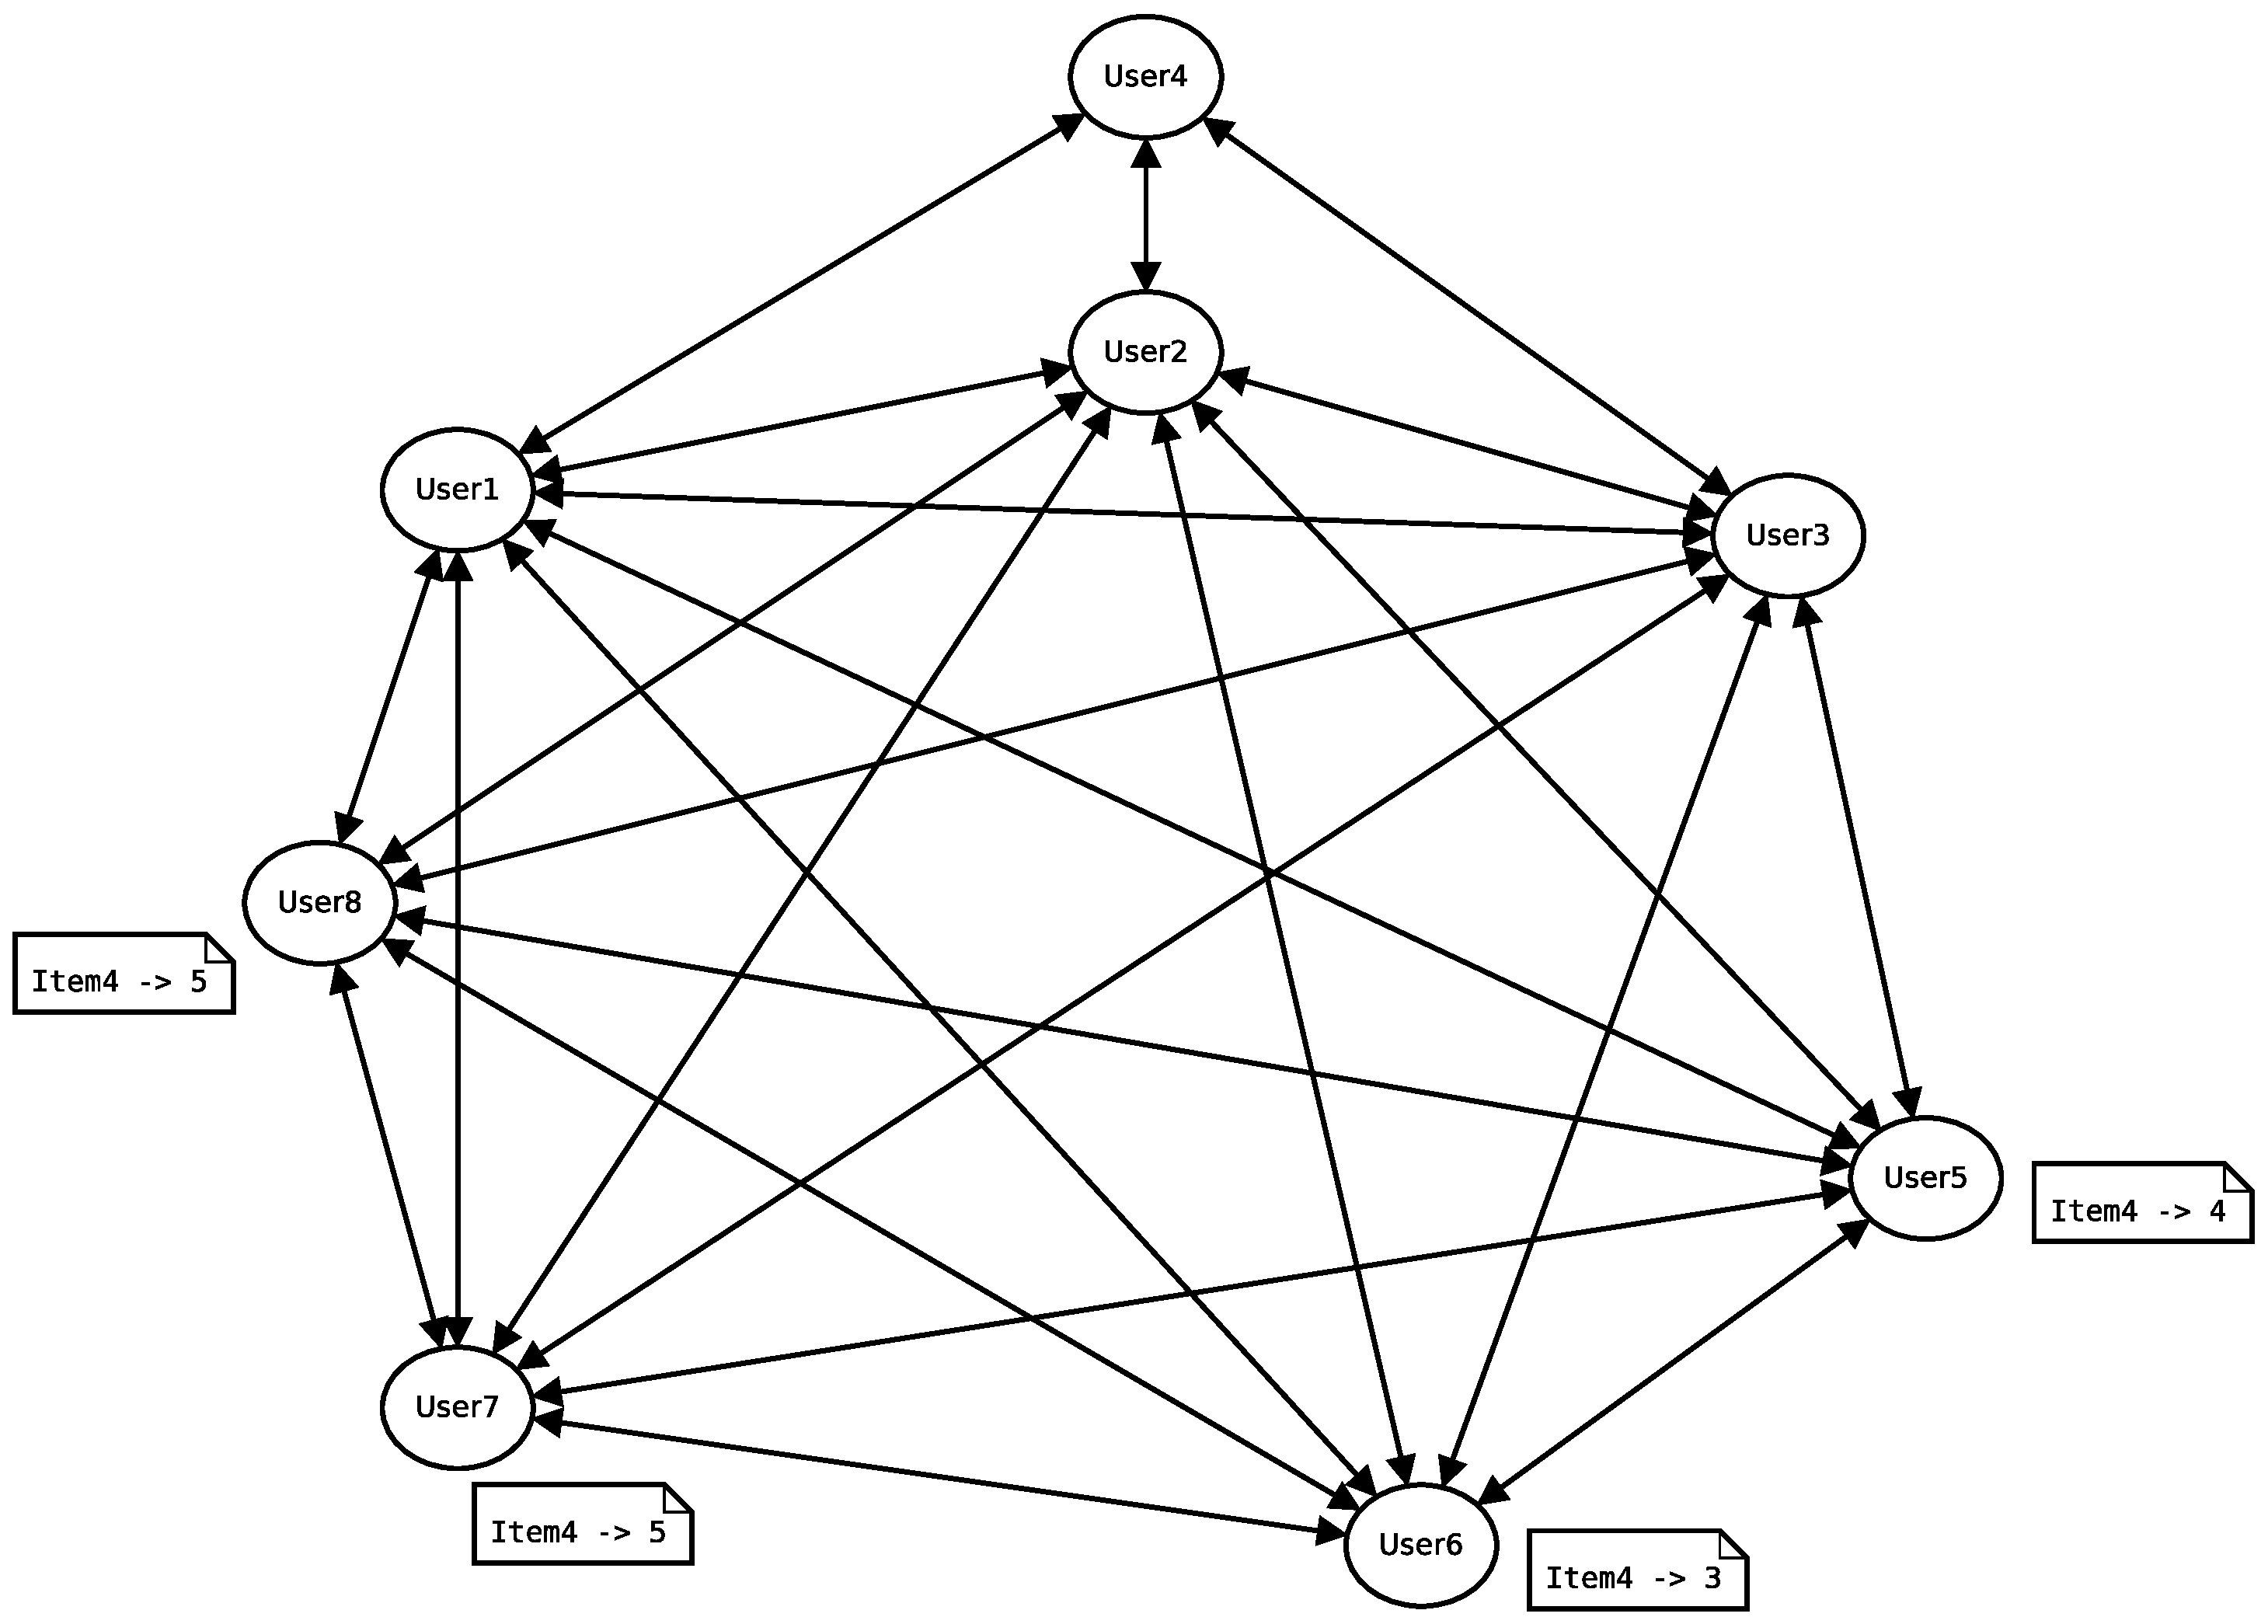
\includegraphics[width=0.95\textwidth]{user_connections.eps}
            \caption{User Connections}
        \end{figure}
    \end{columns}
\end{frame}
\begin{frame}
    \frametitle{Introduction}
    \begin{columns}
        \column{0.5\textwidth}
        \begin{table}
            \centering
            \tiny
            \begin{tabular}{ |c|c|c|c|c|c|c| }
            \hline
            \diagbox{$User$}{$Item$} & \textbf{$Item_1$} & \textbf{$Item_2$} & \textbf{$Item_3$} & \textbf{$Item_4$}  & \textbf{$Item_5$} & \textbf{$Item_6$} \\
            \hline
            \textbf{$User_1$} & 5 & 2 & 3 & {\color{red}4.3} & 1 & 5 \\
            \hline
            \textbf{$User_2$} & 1 & 2 & 4 & {\color{red}4.15} & 2 & 2 \\
            \hline
            \textbf{$User_3$} & 4  & 3 & 5 & {\color{red}4.12} & 4 & 3 \\
            \hline
            \textbf{$User_4$} & 5 & 2 & 3 &  {\color{green}\textbf{?}} & {\color{red}2.35} & {\color{red}3.42} \\
            \hline
            \textbf{$User_5$} & {\color{red}3.35} & {\color{red}2.35}  & {\color{red}4.02} & 4 & 1 & 1 \\
            \hline
            \textbf{$User_6$} & {\color{red}3.21} & {\color{red}2.4} & {\color{red}4.15}  & 3 & 5 & 2 \\
            \hline
            \textbf{$User_7$} & {\color{red}3.46} & {\color{red}2.32} & {\color{red}3.94}  & 5 & 1 & 2 \\
            \hline
            \textbf{$User_8$} & {\color{red}3.36} & {\color{red}2.35} & {\color{red}4.03}  & 5 & 4 & 4 \\
            \hline
            \end{tabular}
            \caption{Ratings Matrix After KNN}
        \end{table}
        \column{0.5\textwidth}
        \vspace{-5mm}
        \begin{figure}
            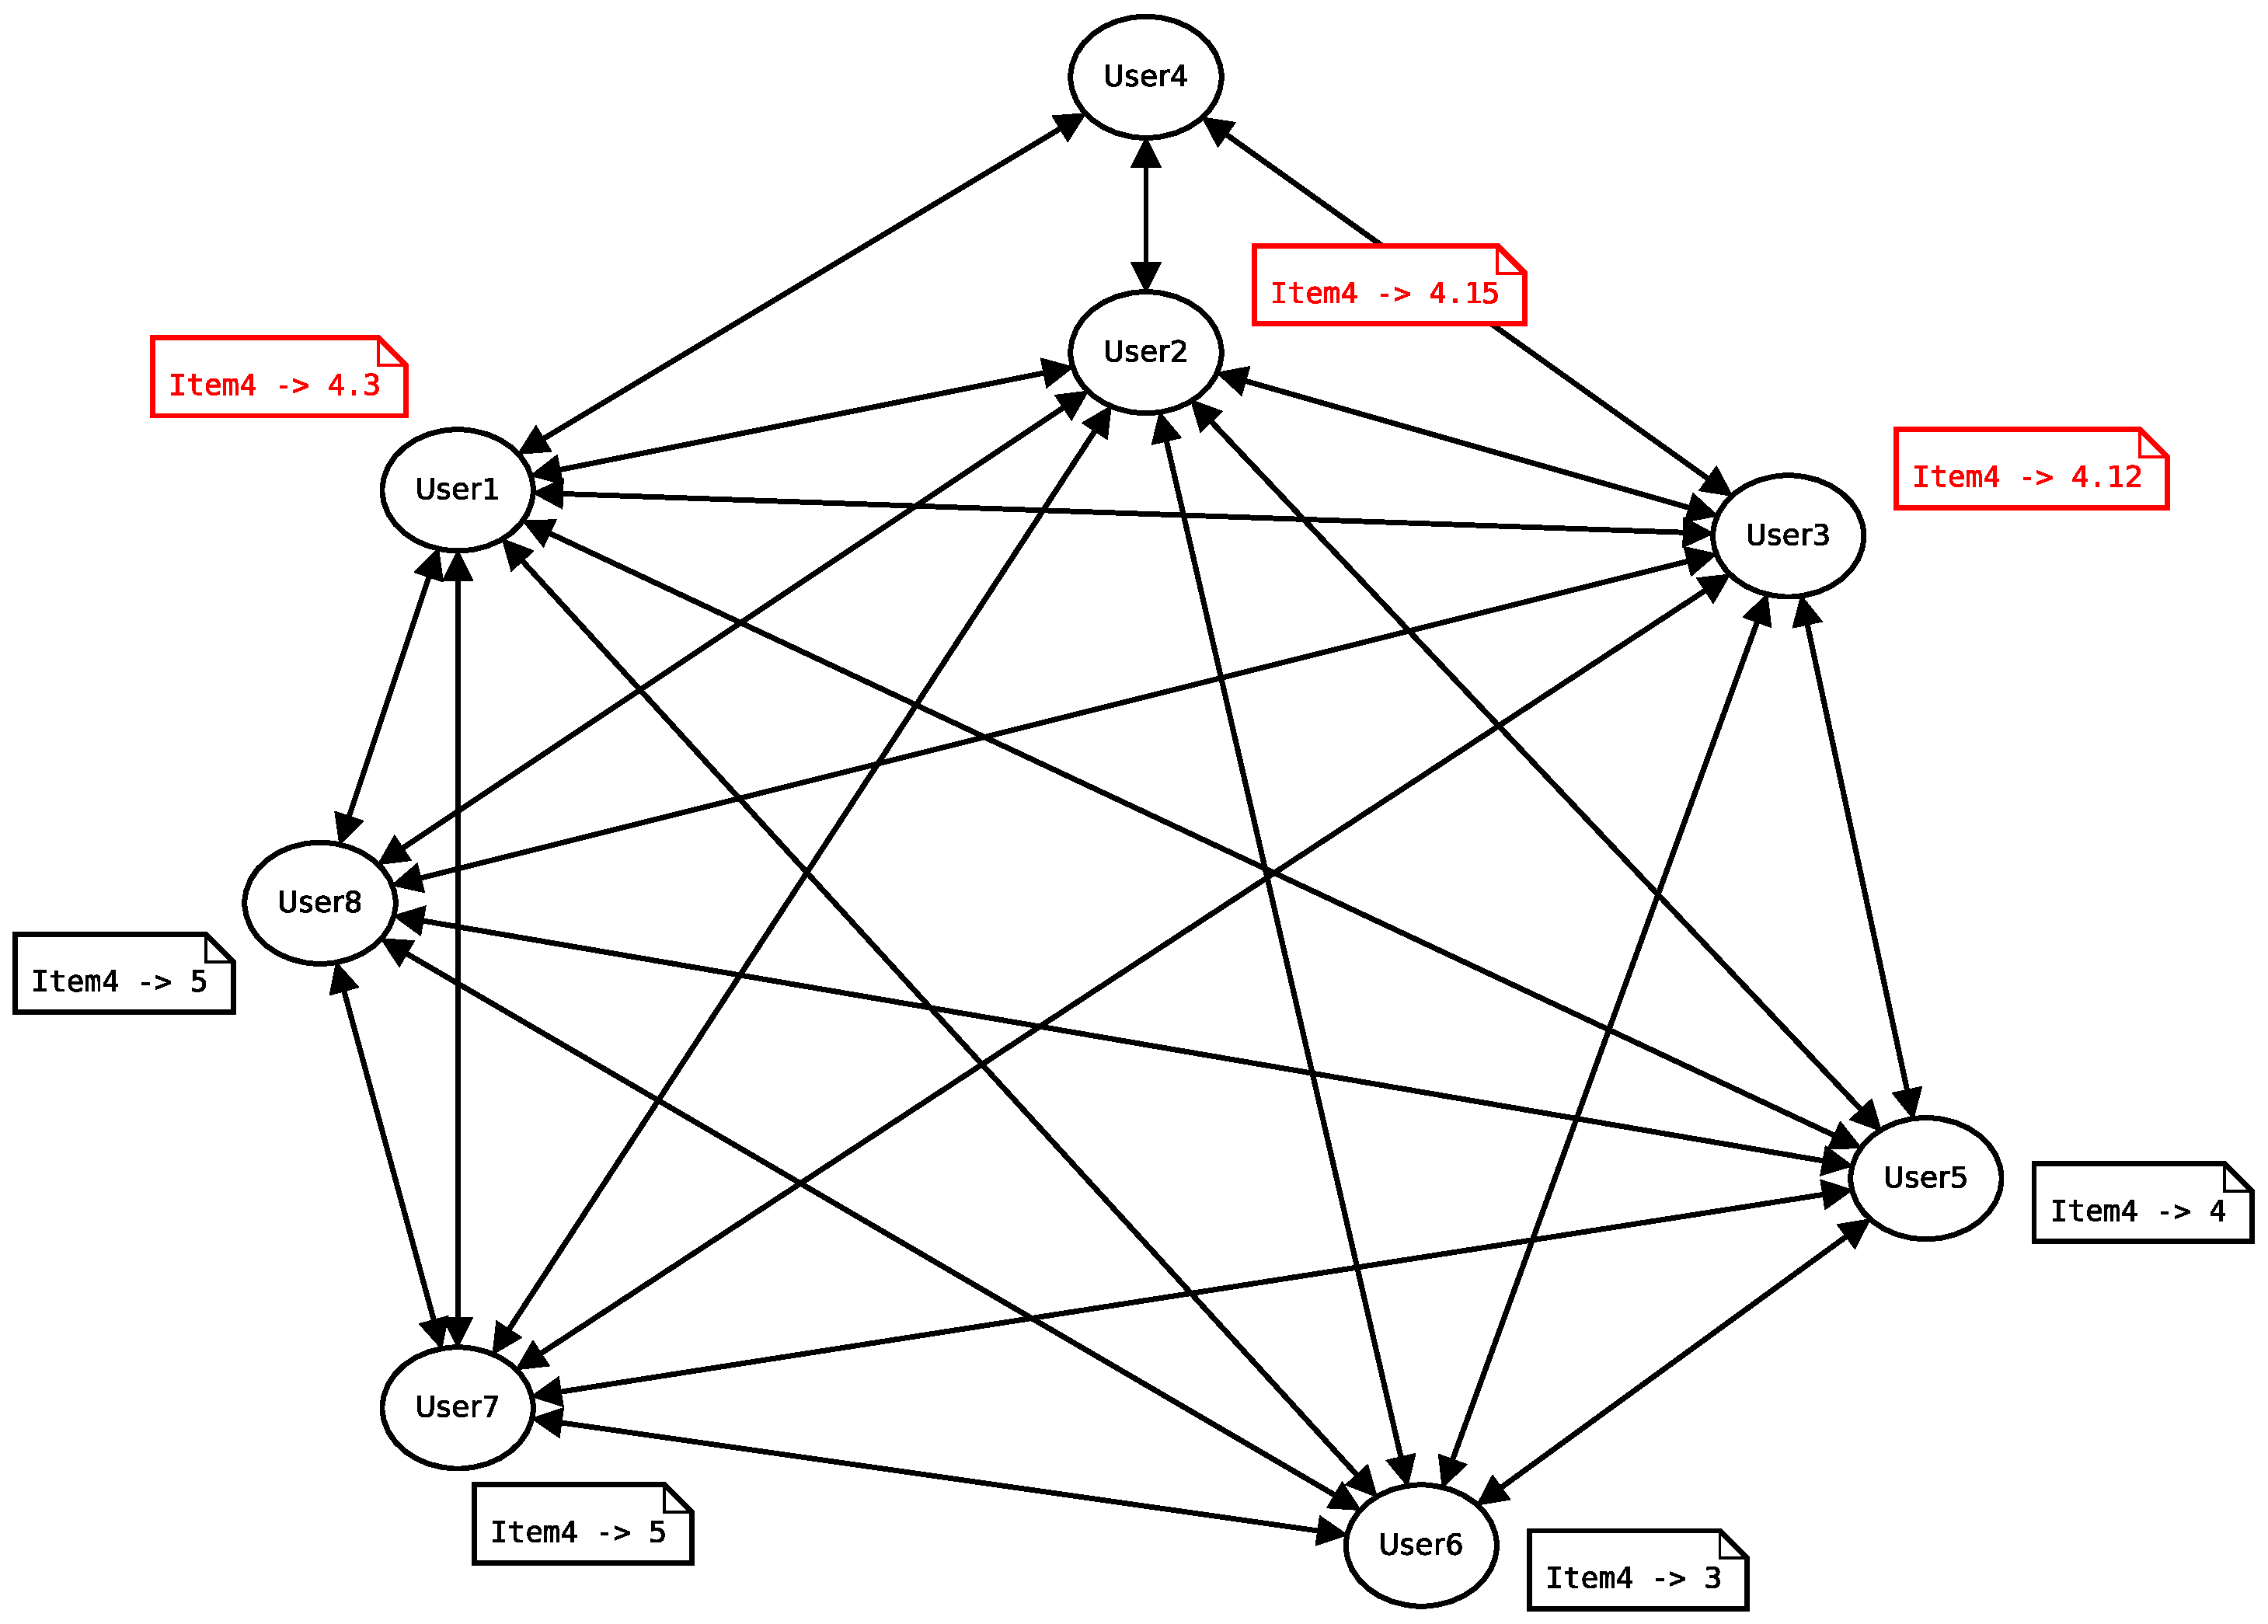
\includegraphics[width=0.95\textwidth]{user_connections_with_KNN.eps}
            \caption{User Connections}
        \end{figure}
    \end{columns}
\end{frame}
\subsection{Methodology}
\begin{frame}
    \frametitle{The Recursive K-Nearest Neighbors Algorithm}
    \only<1>{
        \vspace{2cm}
        \centering
        \textbf{The Recursive K-Nearest Neighbors algorithm}
    }
    \vspace{-1cm}
    \begin{itemize}
    \item[]<2-> \textbf{Step 1:} Select users that have similarity connections with $User_A$, name it $Group_A$.
    \item[]<3-> \textbf{Step 2:} Out of $Group_A$, select those users that have similarity connections with
	other users who have rated $Item_B$, name it $Group_B$.
    \item[]<4-> \textbf{Step 3:}  Sort $Group_B$ in descending order.
    \item[]<5-> \textbf{Step 4:}  Choose how many neighbors from $Group_B$ will contribute in the
	rating prediction by selecting the top $\mathcal{K}$ out of all the available
	neighbors in this group, name it $Group_C$.
    \item[]<6-> \textbf{Step 5:} For each neighbor in $Group_C$, predict how this neighbor would
	rate $Item_B$ using the KNN algorithm. For convenience, call the number of recursive
	neighbors each neighbor in $Group_C$ uses, $\mathcal{M}$-Nearest Neighbors.
    \item[]<7-> \textbf{Step 6:} Perform the KNN algorithm for $User_A$ to $Item_B$
    using the rating predictions applied on $Group_C$.
\end{itemize}
\end{frame}
\begin{frame}
    \frametitle{The Recursive K-Nearest Neighbors Algorithm}
    \vspace{-1cm}
    \begin{columns}
        \column{0.5\textwidth}
        \begin{figure}
        \centering
        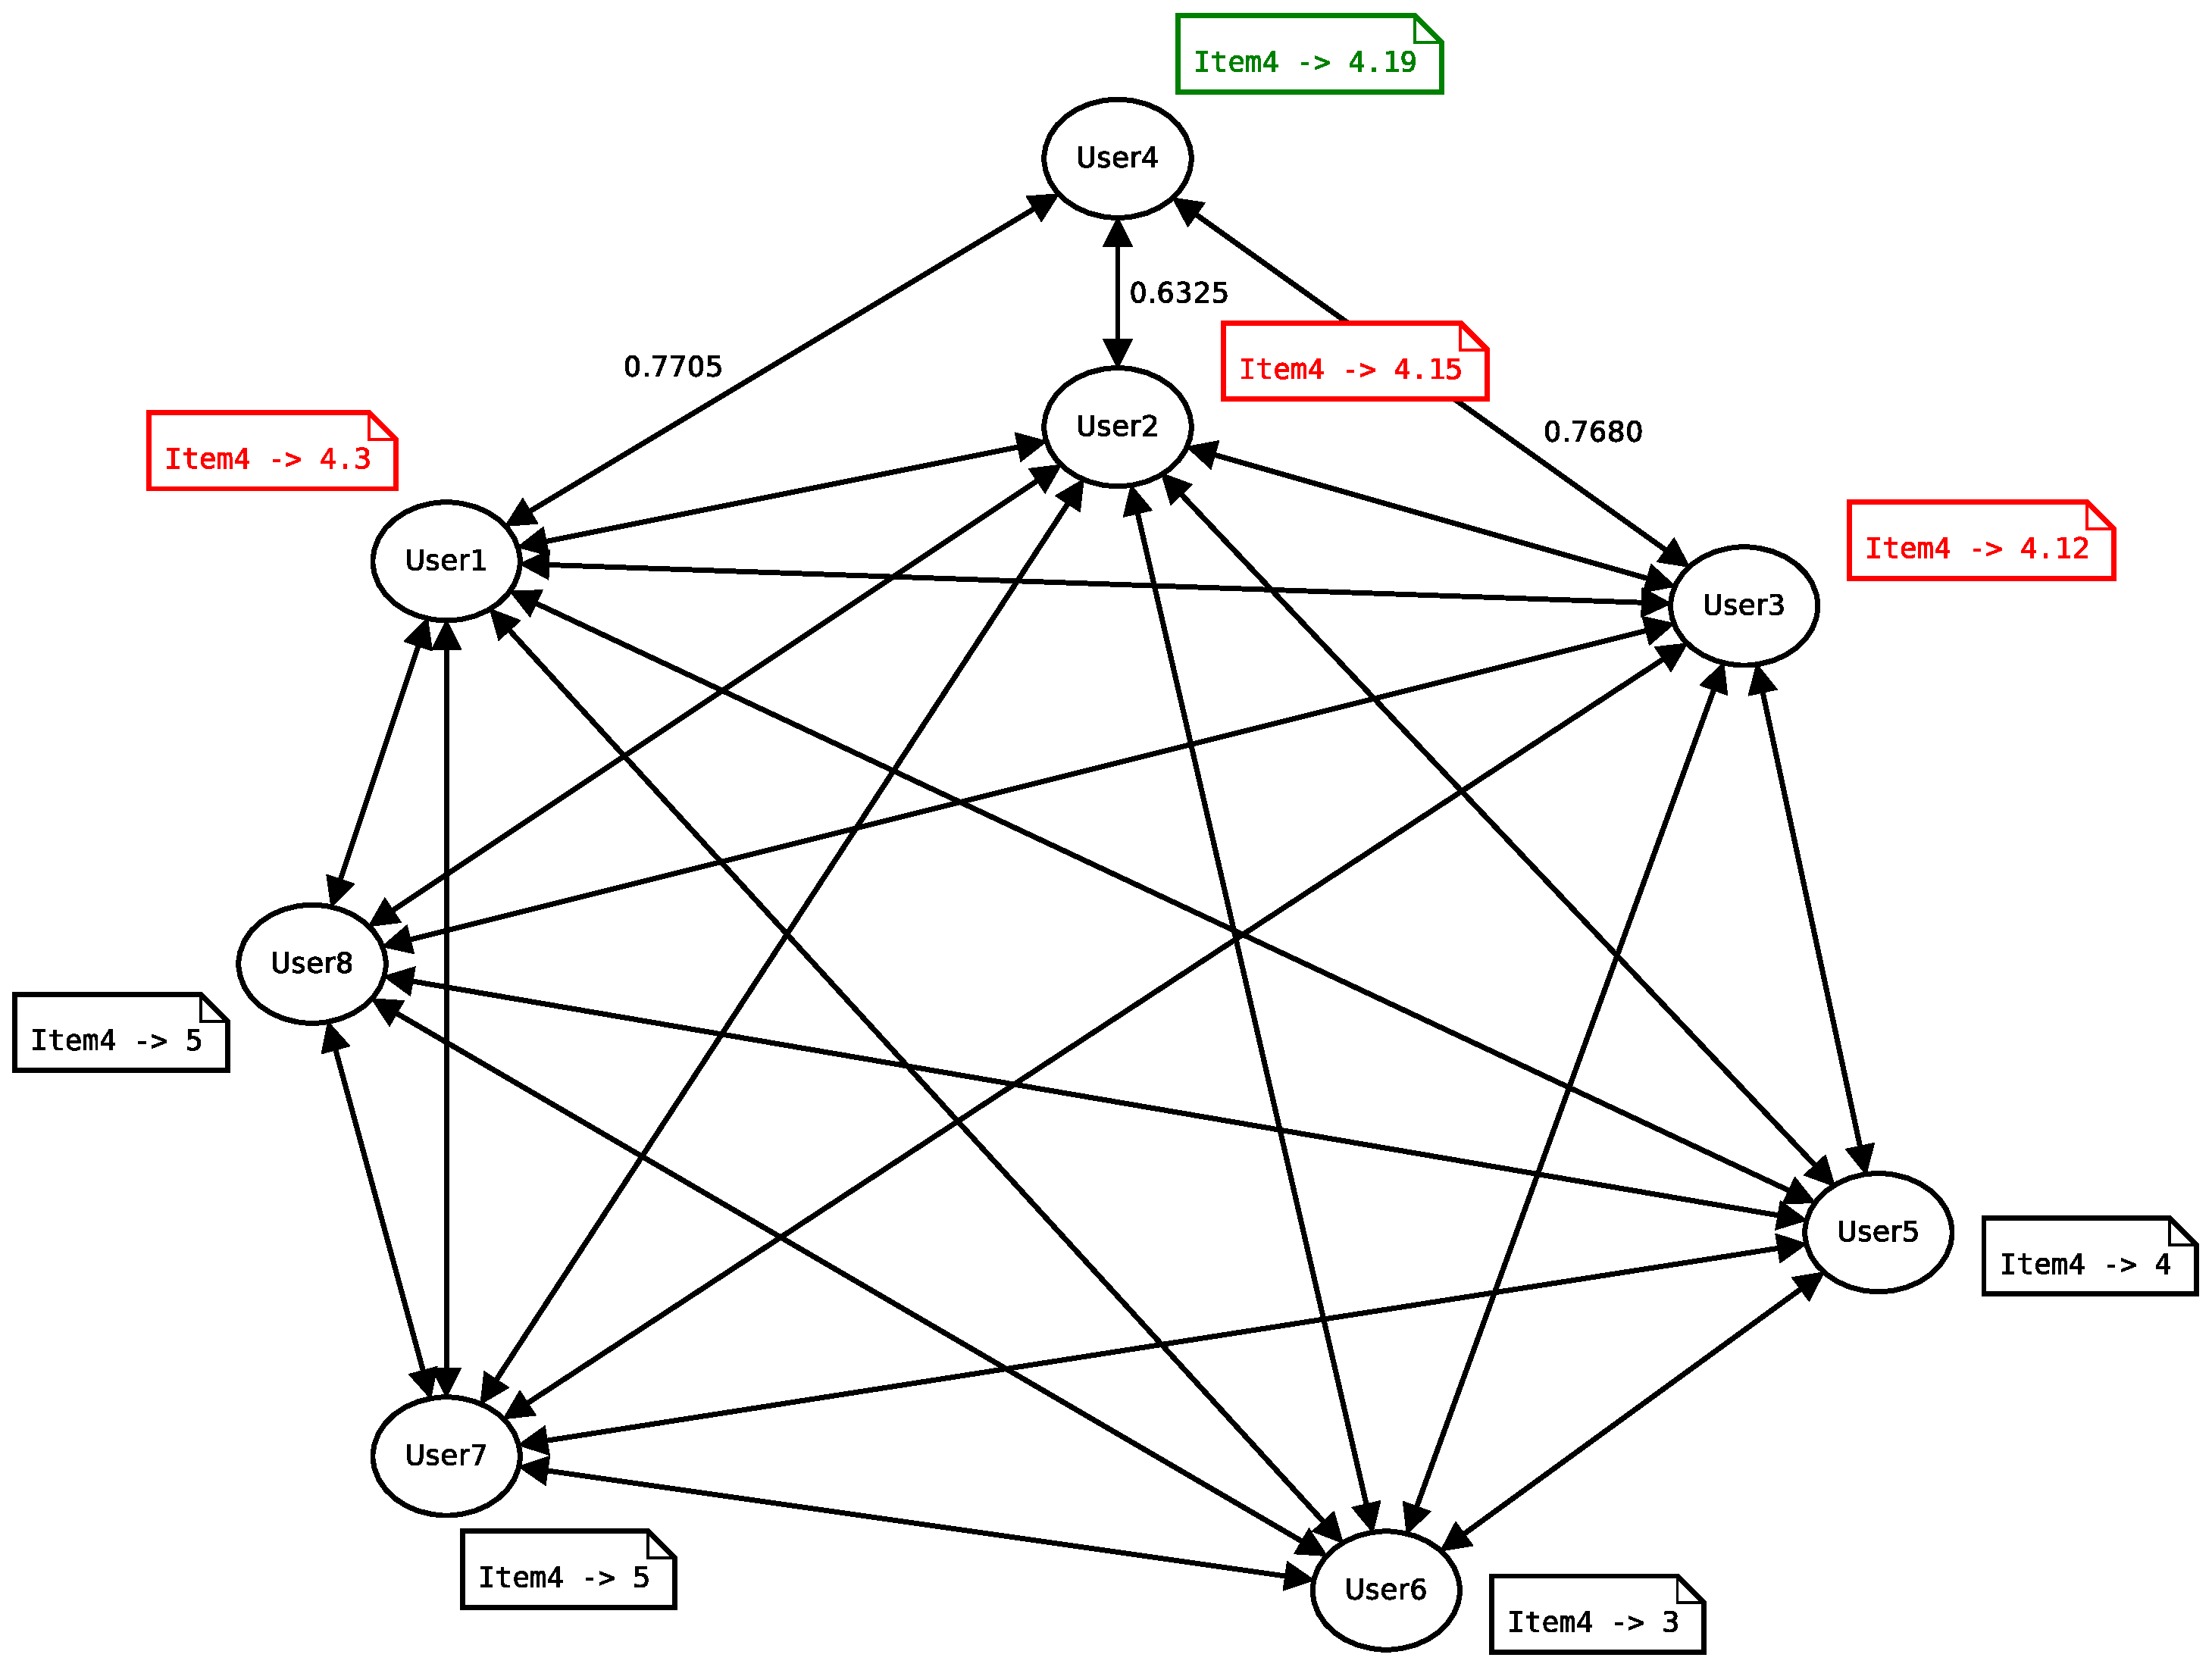
\includegraphics[width=1\textwidth]{RKNN_prediction.eps}
        \end{figure}
        \column{0.5\textwidth}
        \begin{figure}
        \centering
        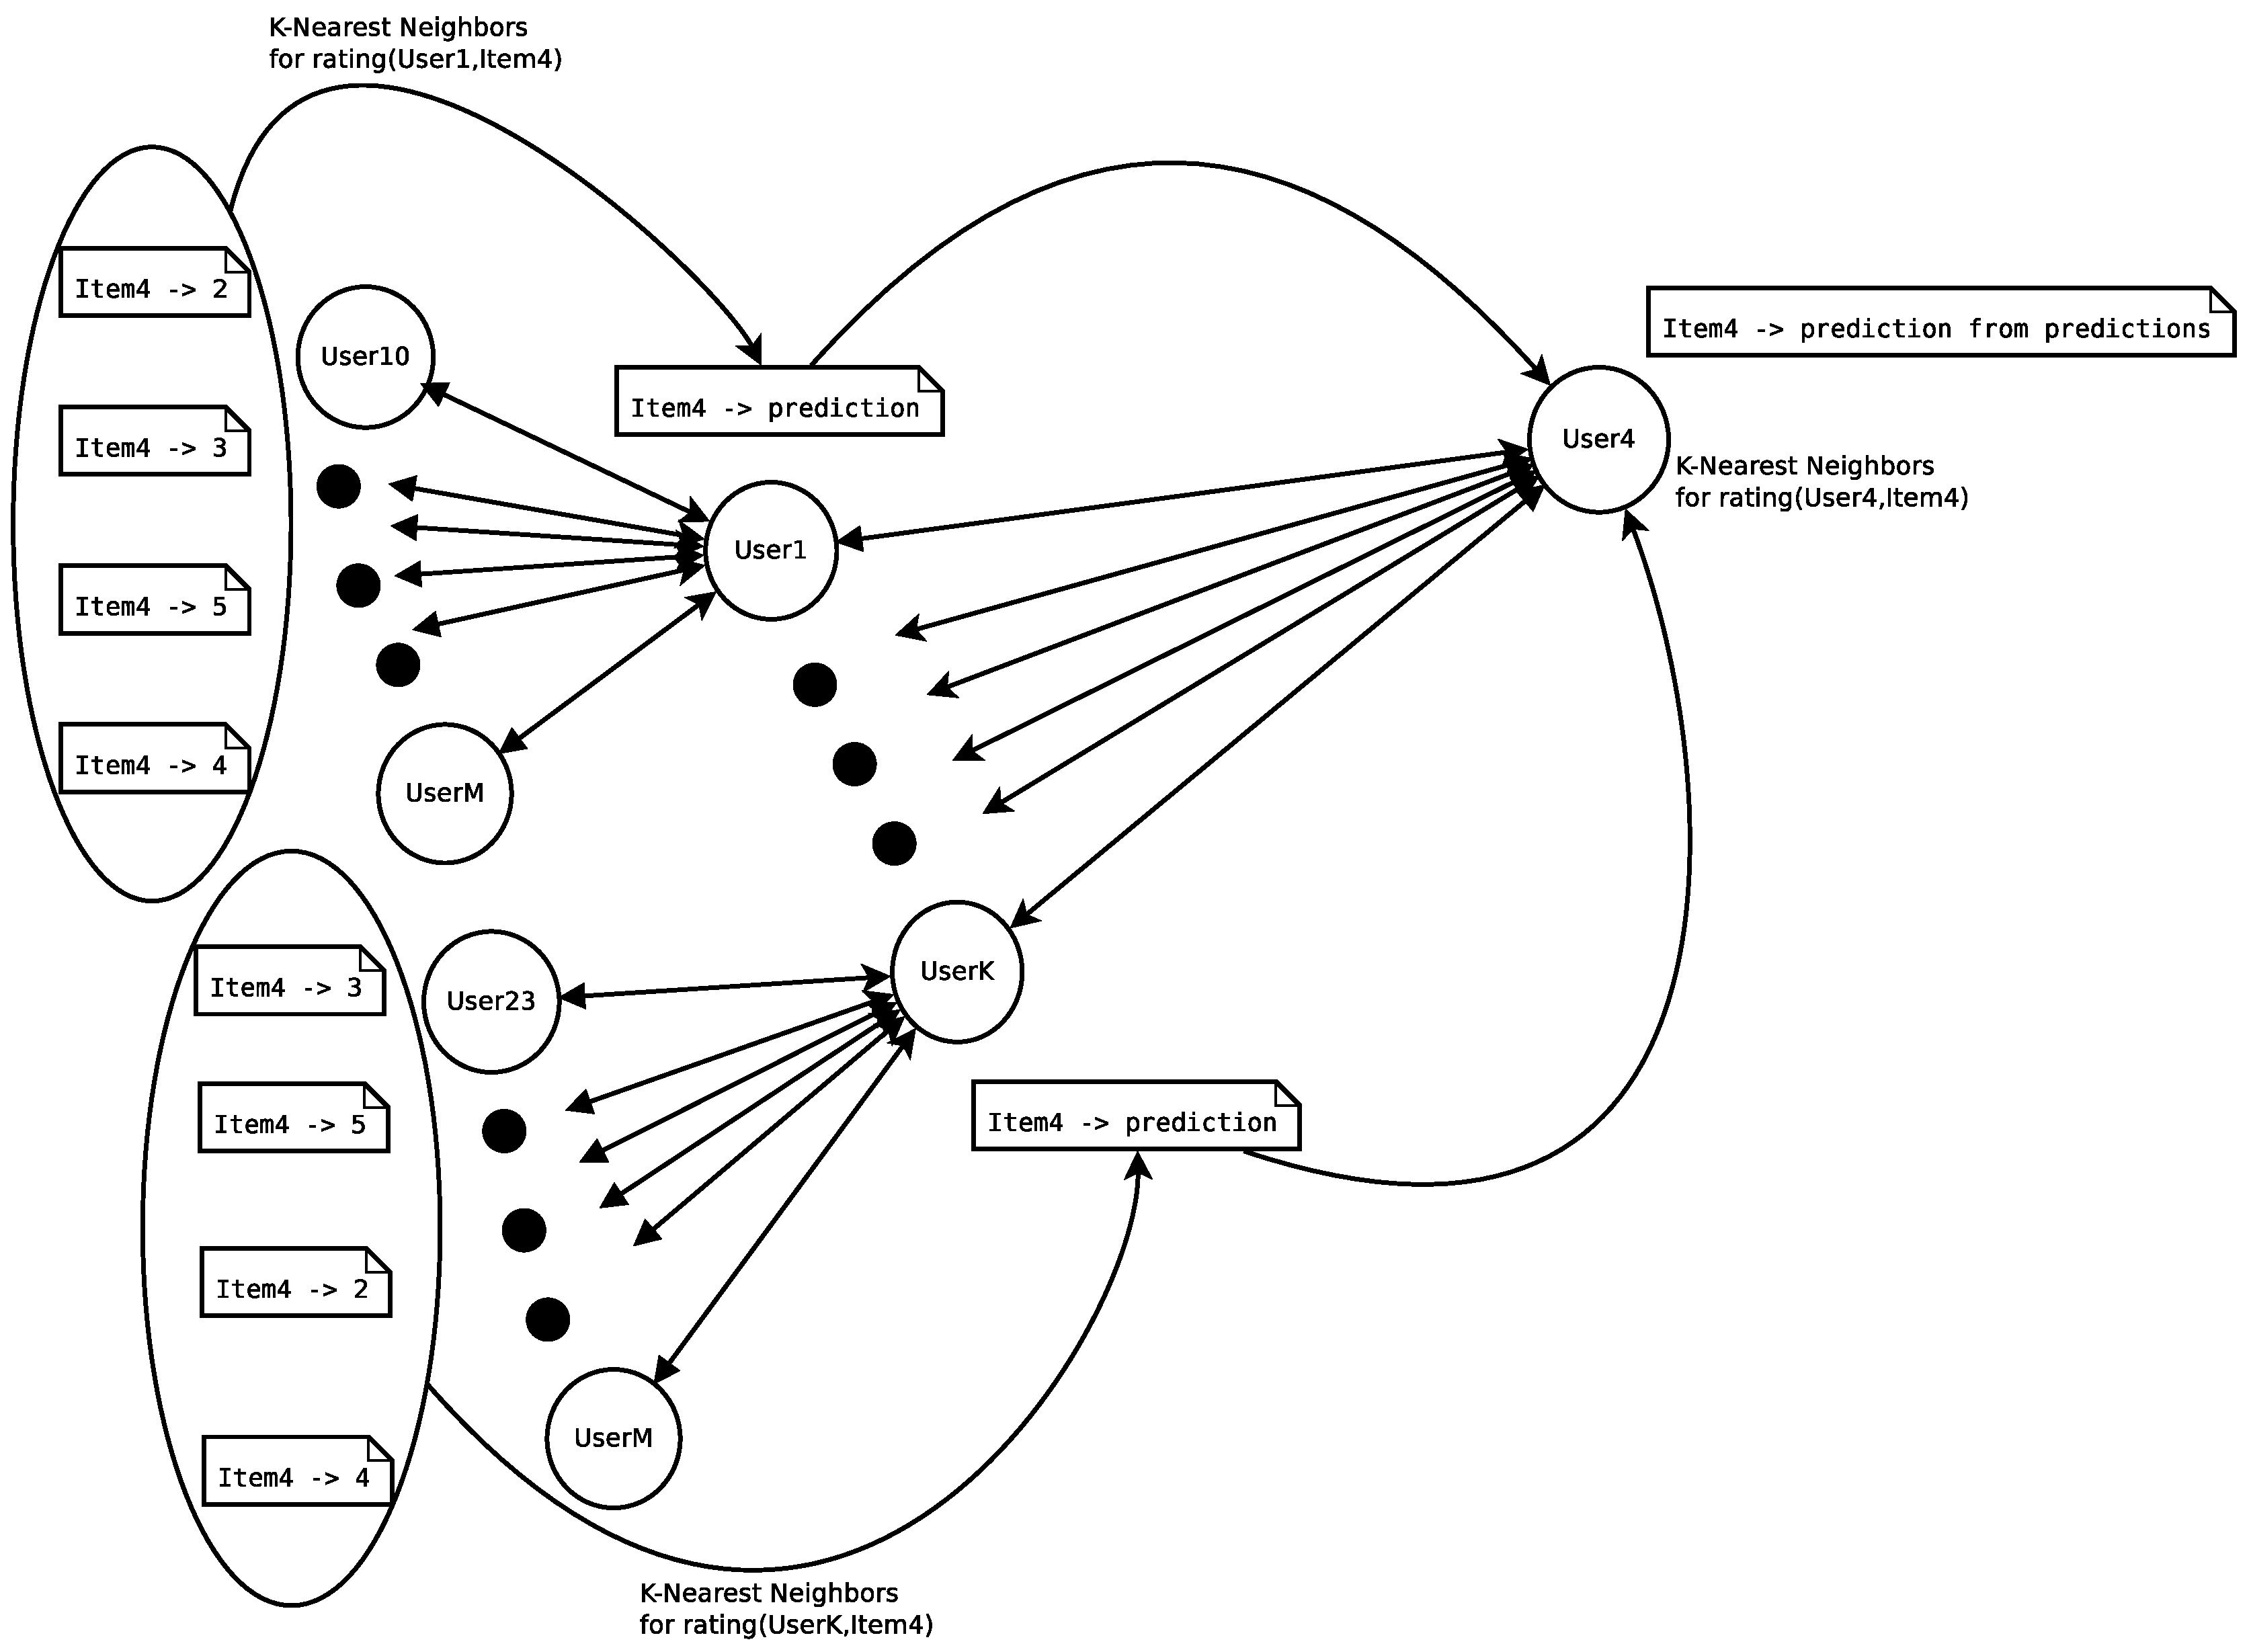
\includegraphics[width=1\textwidth]{Recursive_Nearest_Neighbors.eps}
        \end{figure}
    \end{columns}

\end{frame}

%-----------------------------------------------------------------Results-----------------------------------------------------------------------------------------------------------
% !TeX root = ../main.tex

\section{Results}
\subsection{Data set}
\begin{frame}
    \frametitle{Epinions data set}
    \vspace{-2cm}
    \begin{columns}
    \column{0.5\textwidth}
    \begin{table}
        \centering
        \caption{Epinions Sample}
        \small
        \begin{tabular}{ |c|c|c| }
            \hline
            \textbf{user} & \textbf{item} & \textbf{Rating} \\
            \hline
            36153 & 62461 & 5 \\
            \hline
            427 & 38005 & 5  \\
            \hline
            751 & 53361 & 4 \\
            \hline
            11001 & 118950 & 4 \\
            \hline
            1169 & 66176 & 5 \\
            \hline
            9808 & 84459 & 2 \\
            \hline
            85 & 7446 & 4 \\
            \hline
            14717 & 3397 & 2 \\
            \hline
        \end{tabular}
    \end{table}
    \column{0.5\textwidth}
    \begin{table}
        \centering
        \caption{Epinions Descriptive}
        \small
        \begin{tabular}{ |c|c|c|c| }
            \hline
            &\textbf{Ratings Matrix} & \textbf{Train} & \textbf{Test}\\
            \hline
            count & 664824 & 520203 & 144621\\
            \hline
            mean & 3.9917 & 3.99 & 3.9975\\
            \hline
            std & 1.2068 & 1.2072 & 1.2053\\
            \hline
            min & 1 & 1 & 1\\
            \hline
            25\% & 3 & 3 & 3\\
            \hline
            50\% & 4 & 4 & 4\\
            \hline
            75\% & 5 & 5 & 5\\
            \hline
            max & 5 & 5 & 5\\
            \hline
        \end{tabular}
    \end{table}
\end{columns}
\end{frame}
\subsection{Evaluation Metrics}
\begin{frame}[t]
    \vspace{-1cm}
    \hspace{15mm}\underline{\textbf{Single Model}}  \hspace{5cm}\underline{\textbf{Combined Models}}
    \frametitle{Evaluation Metrics}
    \begin{columns}
    \column{0.4\textwidth}
    \begin{flalign*}
            RMSE &= \sqrt{\frac{\sum_{(u,i) \in \mathcal{T}(r_{u,i} - \hat{r}_{u,i})^2}}{n}} \\
            MAE  &= \frac{\sum_{(u,i) \in \mathcal{T}\left|r_{u,i} - \hat{r}_{u,i}\right|}}{n} \\
            RMSUE &= \frac{1}{n}\sum_{u \in \mathcal{T}}\sqrt{\frac{\sum_{i \in \mathcal{I}_u(r_{u,i} - \hat{r}_{u,i})^2}}{n_u}} \\
            MAUE &= \frac{1}{n}\sum_{u \in \mathcal{T}}\frac{\sum_{i \in \mathcal{I}_u\mathopen|r_{u,i} - \hat{r}_{u,i}\mathclose|}}{n_u}\\
    \end{flalign*}
    \vspace{3cm}
    \column{0.6\textwidth}
    \small
    \begin{flalign*}
        RMSE_{Total} &= \sqrt{\frac{n_{KNN}*RMSE_{KNN}^2 + n_{R-KNN}*RMSE_{R-KNN}^2}{n_{KNN} + n_{R-KNN}}}\\
        MAE_{Total} &= \frac{n_{KNN}*MAE_{KNN} + n_{R-KNN}*MAE_{R-KNN}}{n_{KNN} + n_{R-KNN}}
    \end{flalign*}
    \centering
    \footnotesize
    \begin{itemize}
        \item $\mathcal{T}$ is the test set
        \item $r_{u,i}$ is the truth value of a rating for $user_u$ to $item_i$
        \item $\hat{r_{u,i}}$ is the prediction value of a rating for $user_u$ to $item_i$
        \item $n$ is the number of rating predictions
    \end{itemize}
    \vspace{5cm}
    \end{columns}
\end{frame}

\subsection{Results}
\begin{frame}
    \frametitle{Volume of Predictions}
    \vspace{-1.6cm}
    \begin{table}
\centering
\caption{Ratings Predicted with KNN and Recursive-KNN}
\footnotesize
\begin{tabular}{ccc|ccc|c}
\multicolumn{3}{c|}{\textbf{USERS}}            & \multicolumn{3}{c|}{\textbf{ITEMS}}            &                          \\ \cline{1-6}
\textbf{KNN} & \textbf{R-KNN} & \textbf{TOTAL} & \textbf{KNN} & \textbf{R-KNN} & \textbf{TOTAL} & \textbf{SIMILARITY}      \\ \hline
88379        & 34392          & 122771         & 89800        & 33315          & 123115         & Adjusted Cosine          \\
100311       & 24122          & 124433         & 100311       & 24122          & 124433         & Cosine                   \\
100311       & 24122          & 124433         & 100311       & 24122          & 124433         & Jaccard                  \\
93924        & 29747          & 123671         & 94528        & 29203          & 123731         & MAD                      \\
93924        & 29747          & 123671         & 94528        & 29203          & 123731         & MSD                      \\
88379        & 34392          & 122771         & 89800        & 33315          & 123115         & Modified Adjusted Cosine \\
100311       & 24122          & 124433         & 100311       & 24122          & 124433         & Modified Cosine          \\
59017        & 40470          & 99487          & 54644        & 34096          & 88740          & Modified Pearson 1       \\
89936        & 28183          & 118119         & 84511        & 24357          & 108868         & Modified Pearson 2       \\
89936        & 28183          & 118119         & 84511        & 24357          & 108868         & Pearson
\end{tabular}
\end{table}
\end{frame}
\begin{frame}[t]
    \frametitle{User-based KNN and Total RMSE}
    \vspace{-0.7cm}
    \begin{columns}
        \column{0.5\textwidth}
        \centering
        \underline{\textbf{KNN}}
    \begin{figure}
    \centering
    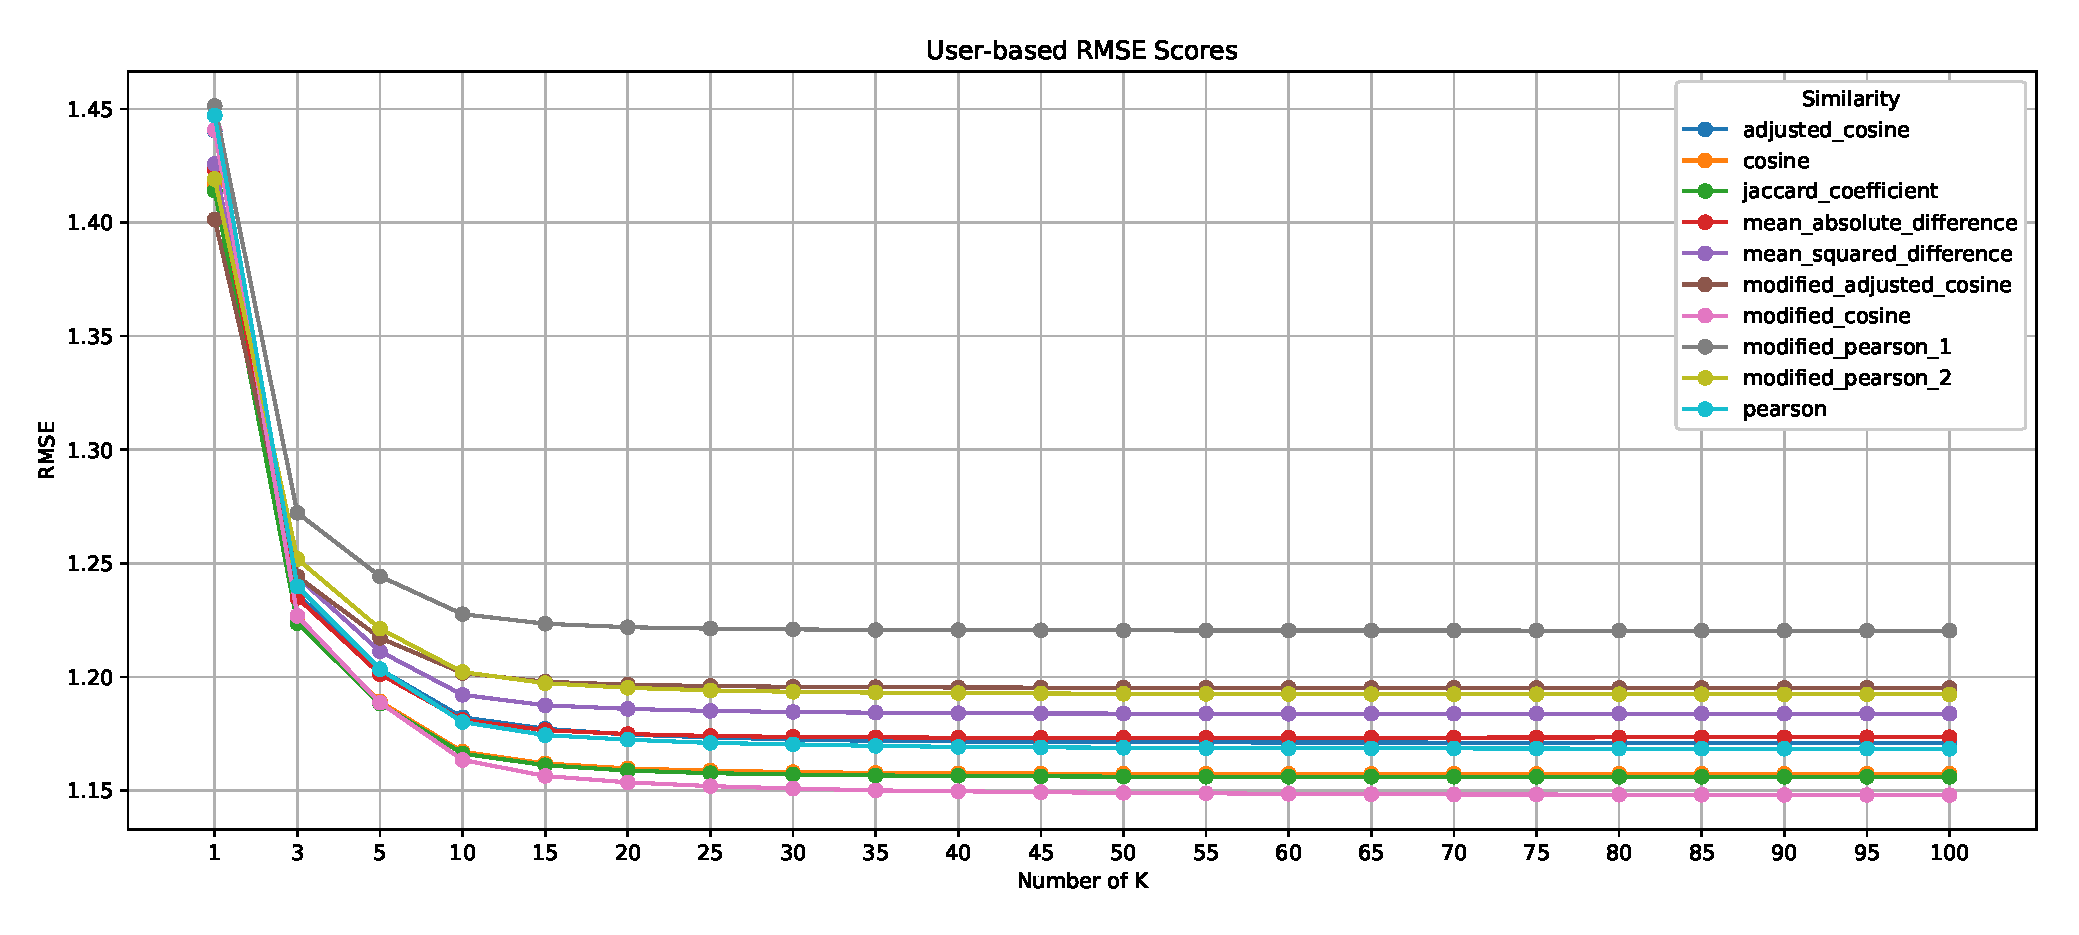
\includegraphics[width=1\textwidth,height=0.6\textheight]{User_RMSE_KNN.eps}
    \end{figure}
    \centering
    \tiny
    Modified cosine at K=100, RMSE=1.1479835373
        \column{0.5\textwidth}
        \centering
        \underline{\textbf{Total}}
    \begin{figure}
    \centering
    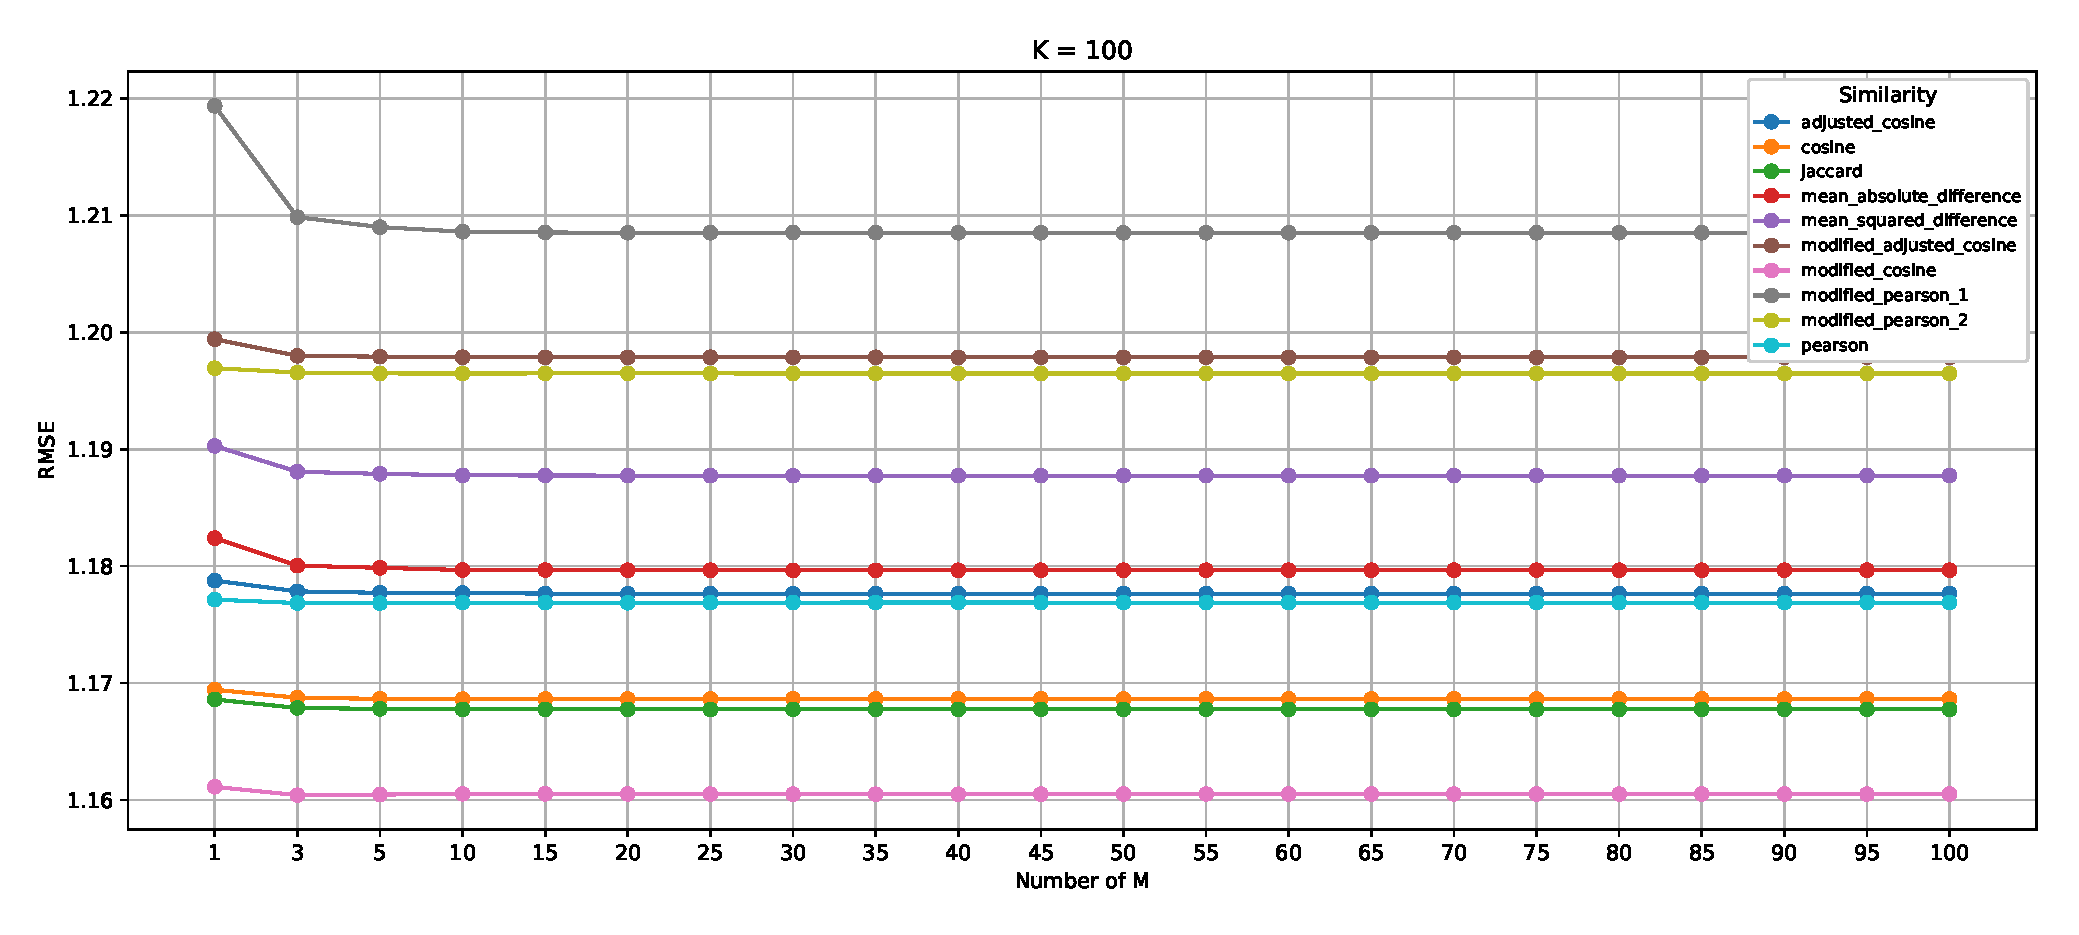
\includegraphics[width=1\textwidth,height=0.6\textheight]{evaluation_user_rmse.eps}
    \end{figure}
    \centering
    \tiny
    Modified cosine at K=100 \& M=3, RMSE=1.1604146071
\end{columns}
\end{frame}
\begin{frame}[t]
    \frametitle{User-based KNN and Total MAE}
        \vspace{-0.7cm}
        \begin{columns}
            \column{0.5\textwidth}
            \centering
            \underline{\textbf{KNN}}
        \begin{figure}
        \centering
        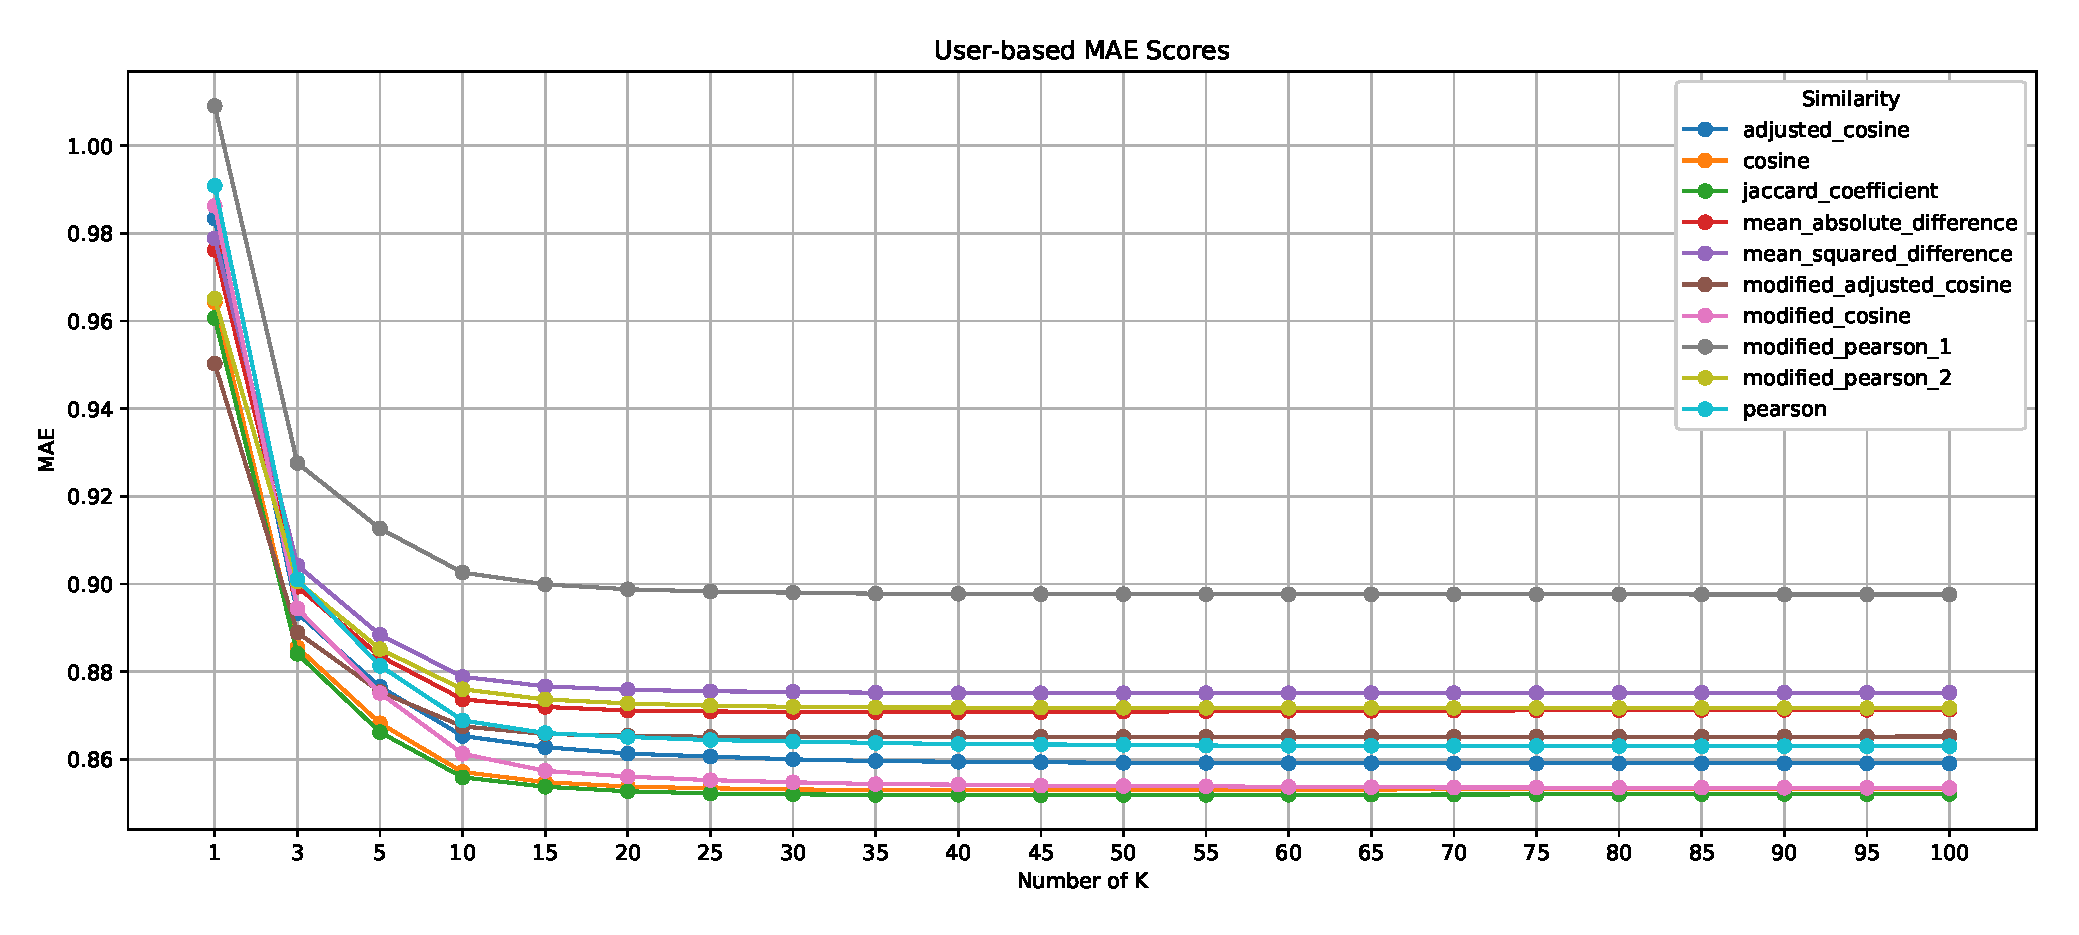
\includegraphics[width=1\textwidth,height=0.6\textheight]{User_MAE_KNN.eps}
        \end{figure}
        \centering
        \tiny
        Jaccard coefficient at K=50, MAE=0.8518433005
            \column{0.5\textwidth}
            \centering
            \underline{\textbf{Total}}
        \begin{figure}
        \centering
        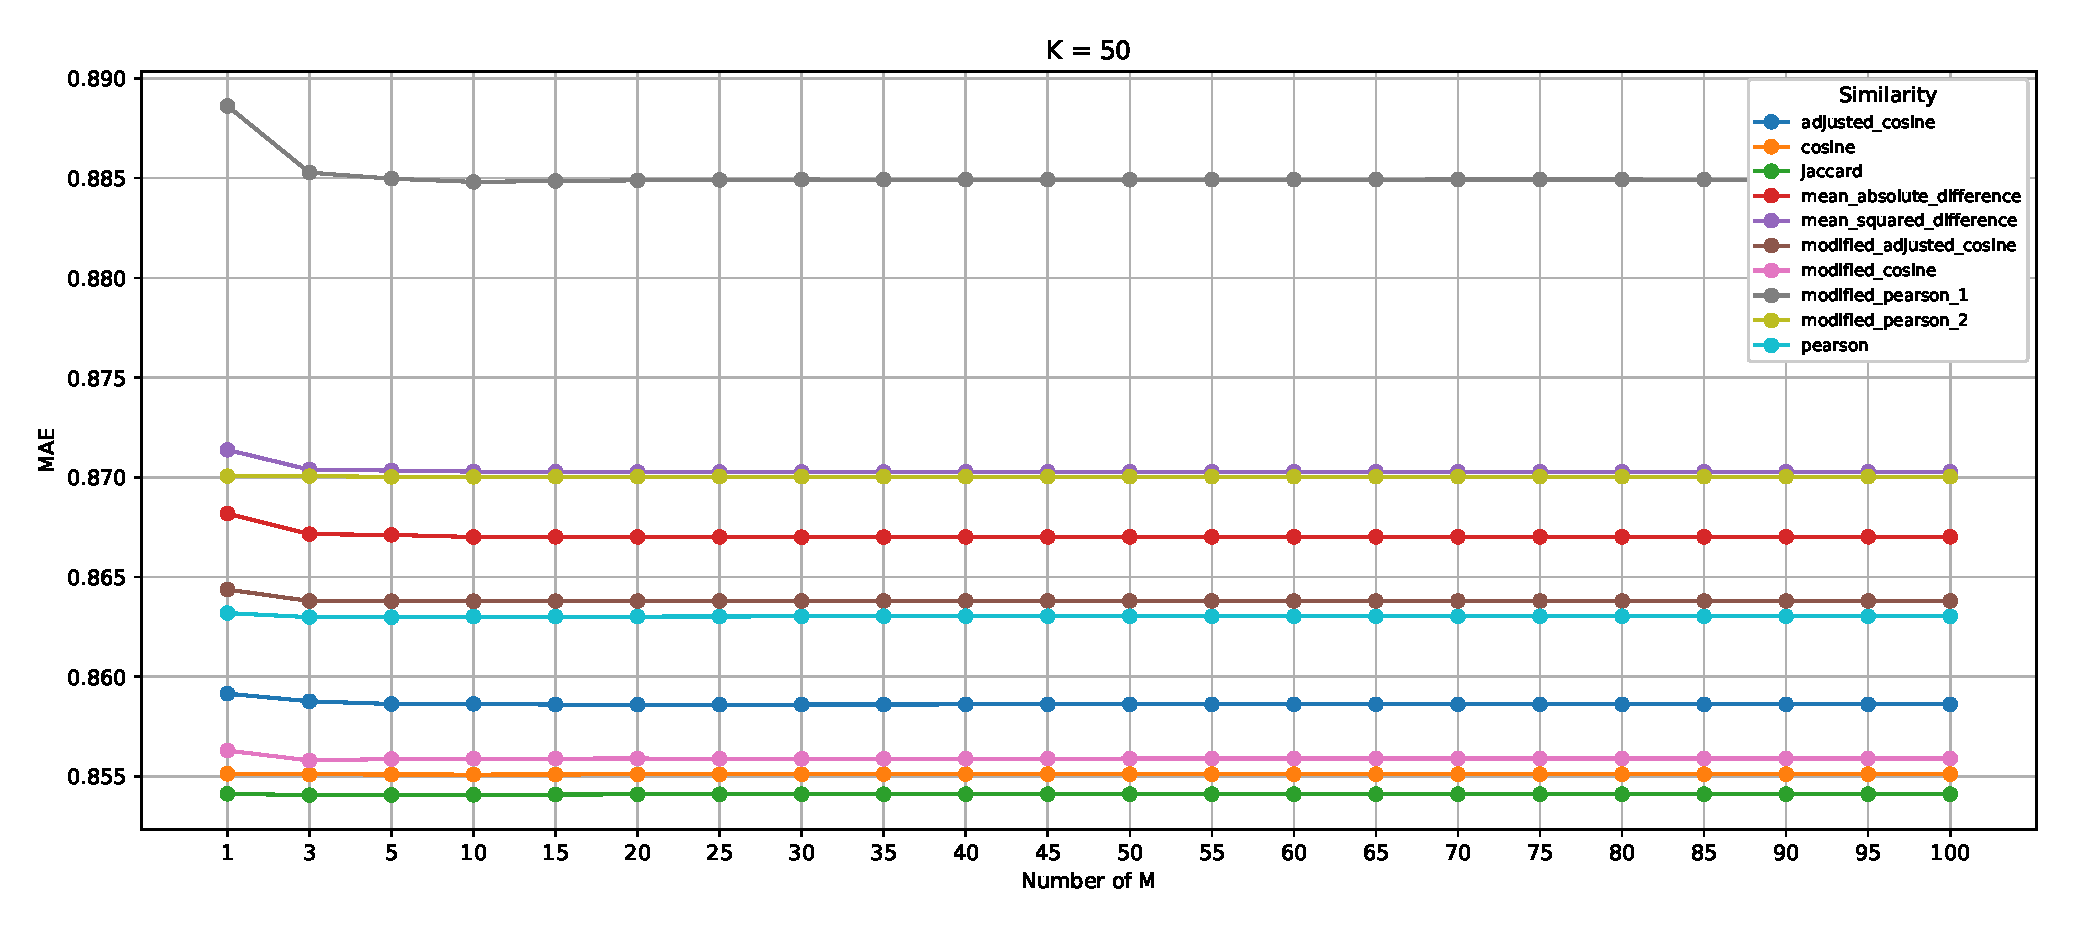
\includegraphics[width=1\textwidth,height=0.6\textheight]{evaluation_user_mae.eps}
        \end{figure}
        \centering
        \tiny
        Jaccard coefficient at K=50 \& M=3, MAE=0.854066176
    \end{columns}
\end{frame}
\begin{frame}[t]
    \frametitle{User-based KNN and Recursive-KNN RMSUE}
    \vspace{-0.7cm}
    \begin{columns}
        \column{0.5\textwidth}
        \centering
        \underline{\textbf{KNN}}
    \begin{figure}
    \centering
    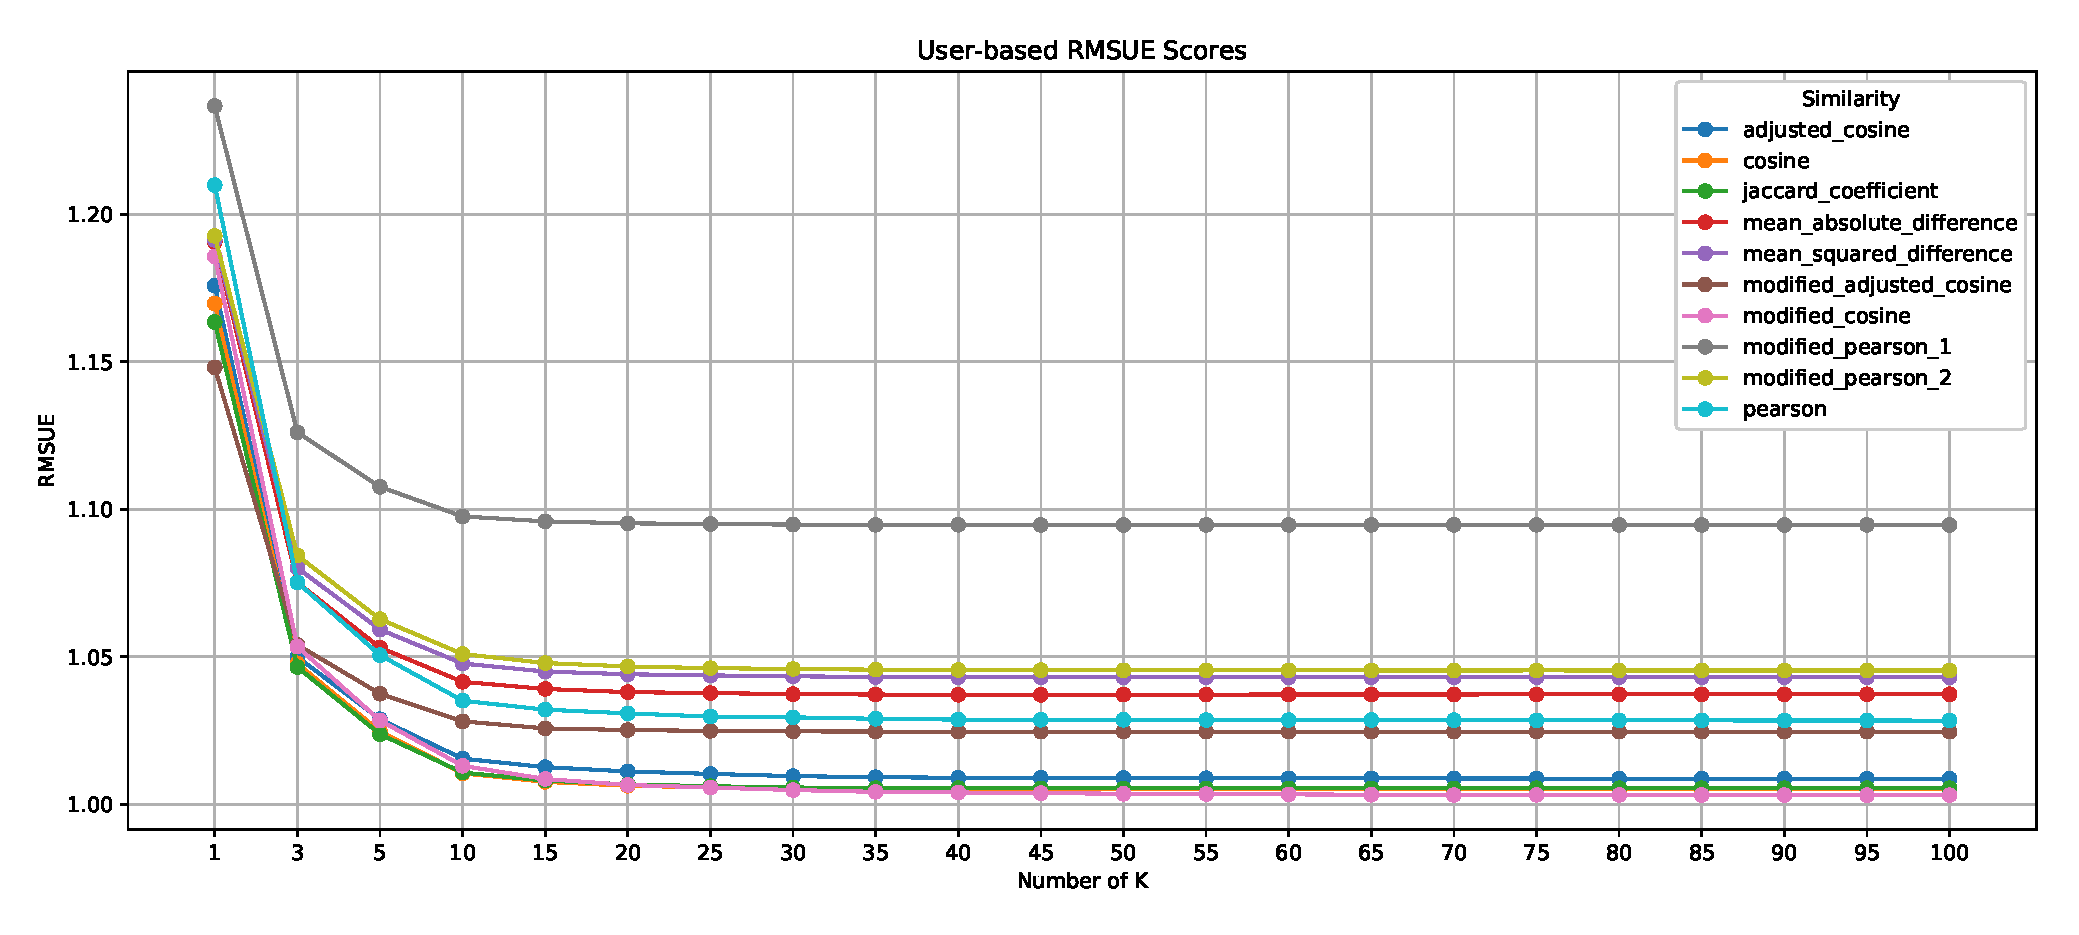
\includegraphics[width=1\textwidth,height=0.6\textheight]{User_RMSUE_KNN.eps}
    \end{figure}
    \centering
    \tiny
    Modified cosine at K=100, RMSUE=1.0031145695
        \column{0.5\textwidth}
        \centering
        \underline{\textbf{Recursive-KNN}}
    \begin{figure}
    \centering
    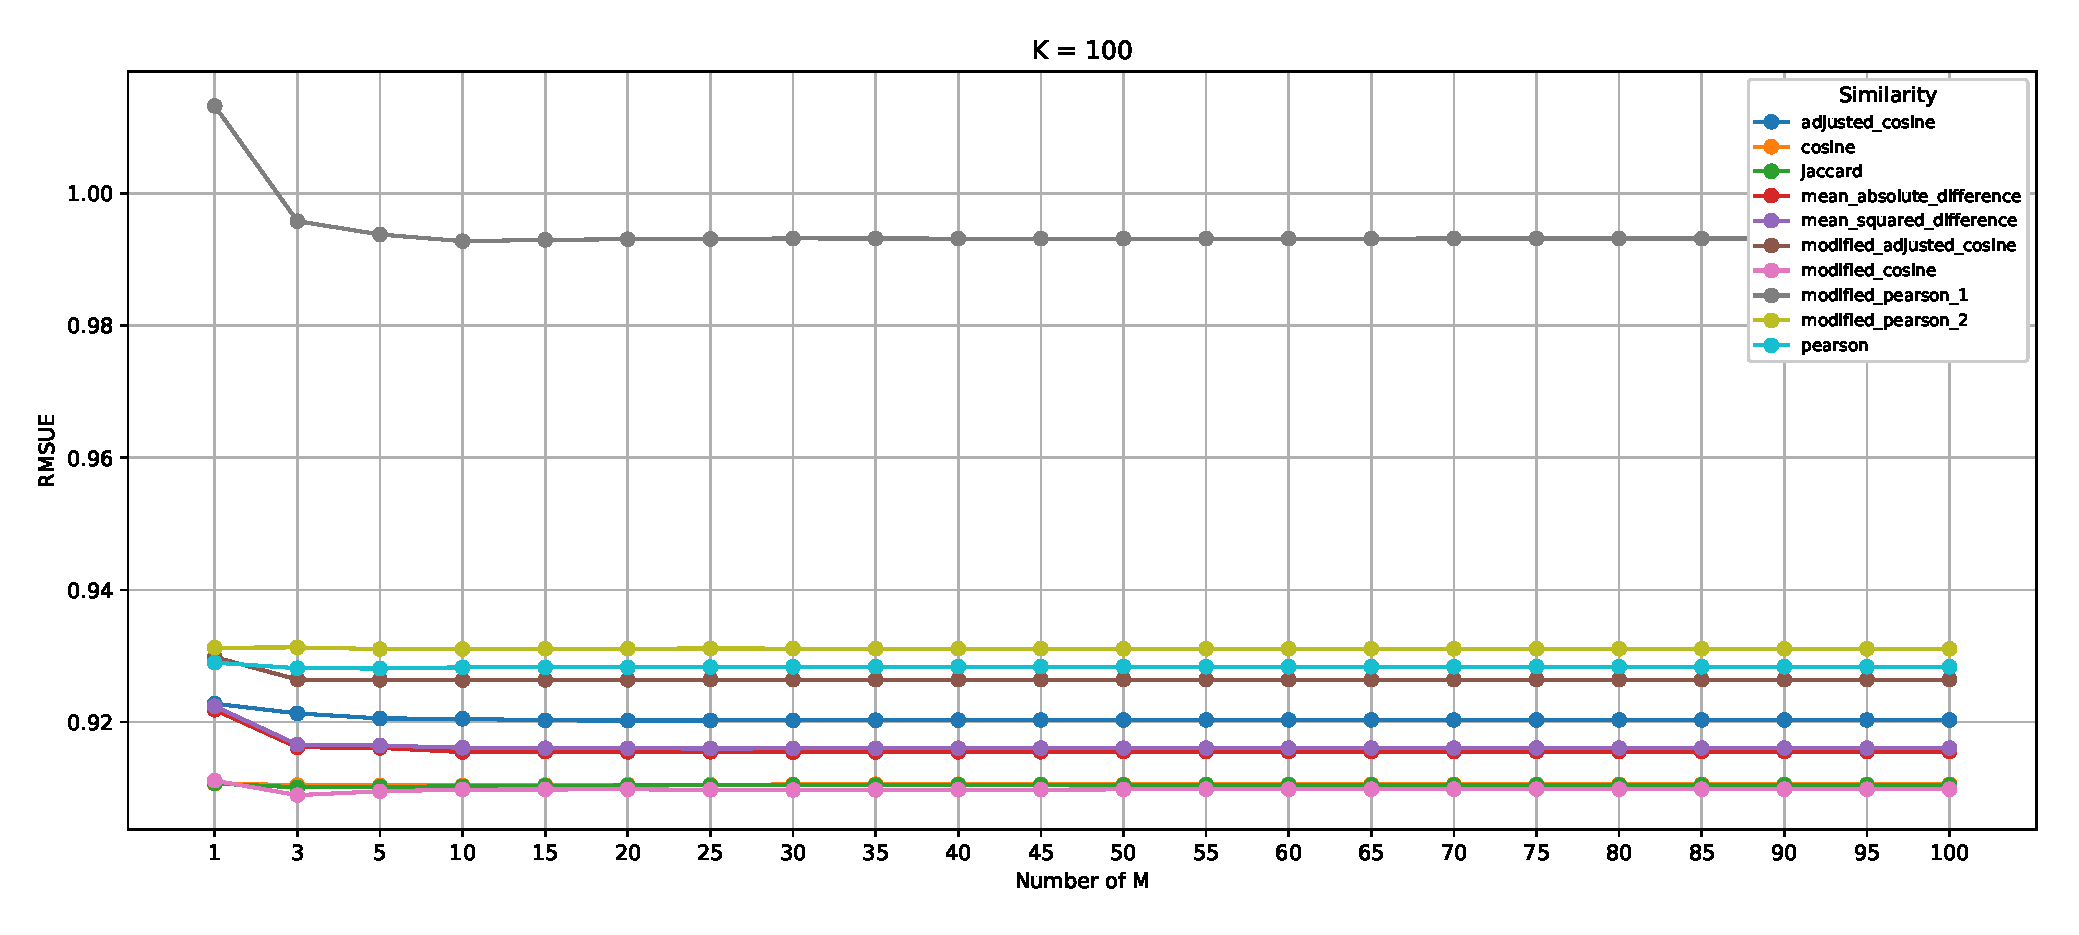
\includegraphics[width=1\textwidth,height=0.6\textheight]{evaluation_user_rmsue.eps}
    \end{figure}
    \centering
    \tiny
    Modified cosine at K=100 \& M=3, RMSUE=0.9089525549
\end{columns}
\end{frame}
\begin{frame}[t]
    \frametitle{User-based KNN and Recursive-KNN MAUE}
    \vspace{-0.7cm}
    \begin{columns}
        \column{0.5\textwidth}
        \centering
        \underline{\textbf{KNN}}
    \begin{figure}
    \centering
    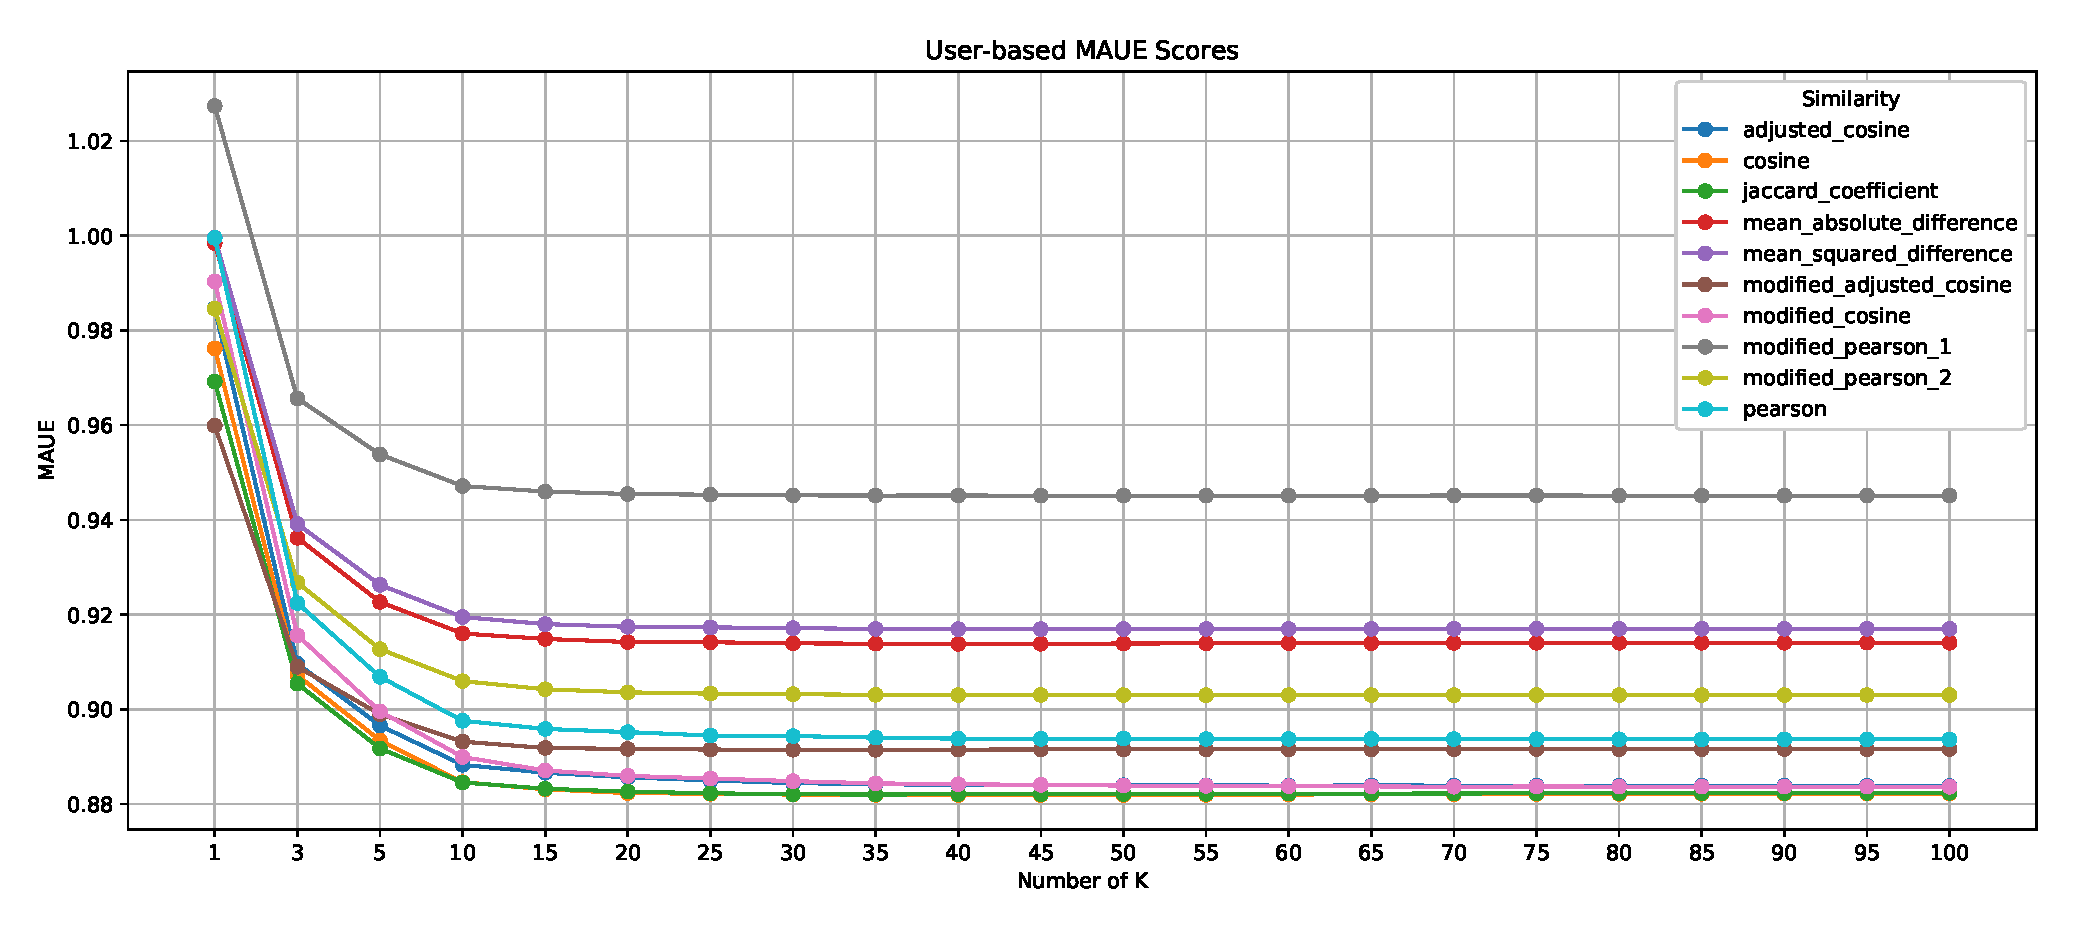
\includegraphics[width=1\textwidth,height=0.6\textheight]{User_MAUE_KNN.eps}
    \end{figure}
    \centering
    \tiny
    Cosine similarity at K=50, MAUE=0.8819077974
        \column{0.5\textwidth}
        \centering
        \underline{\textbf{Recursive-KNN}}
    \begin{figure}
    \centering
    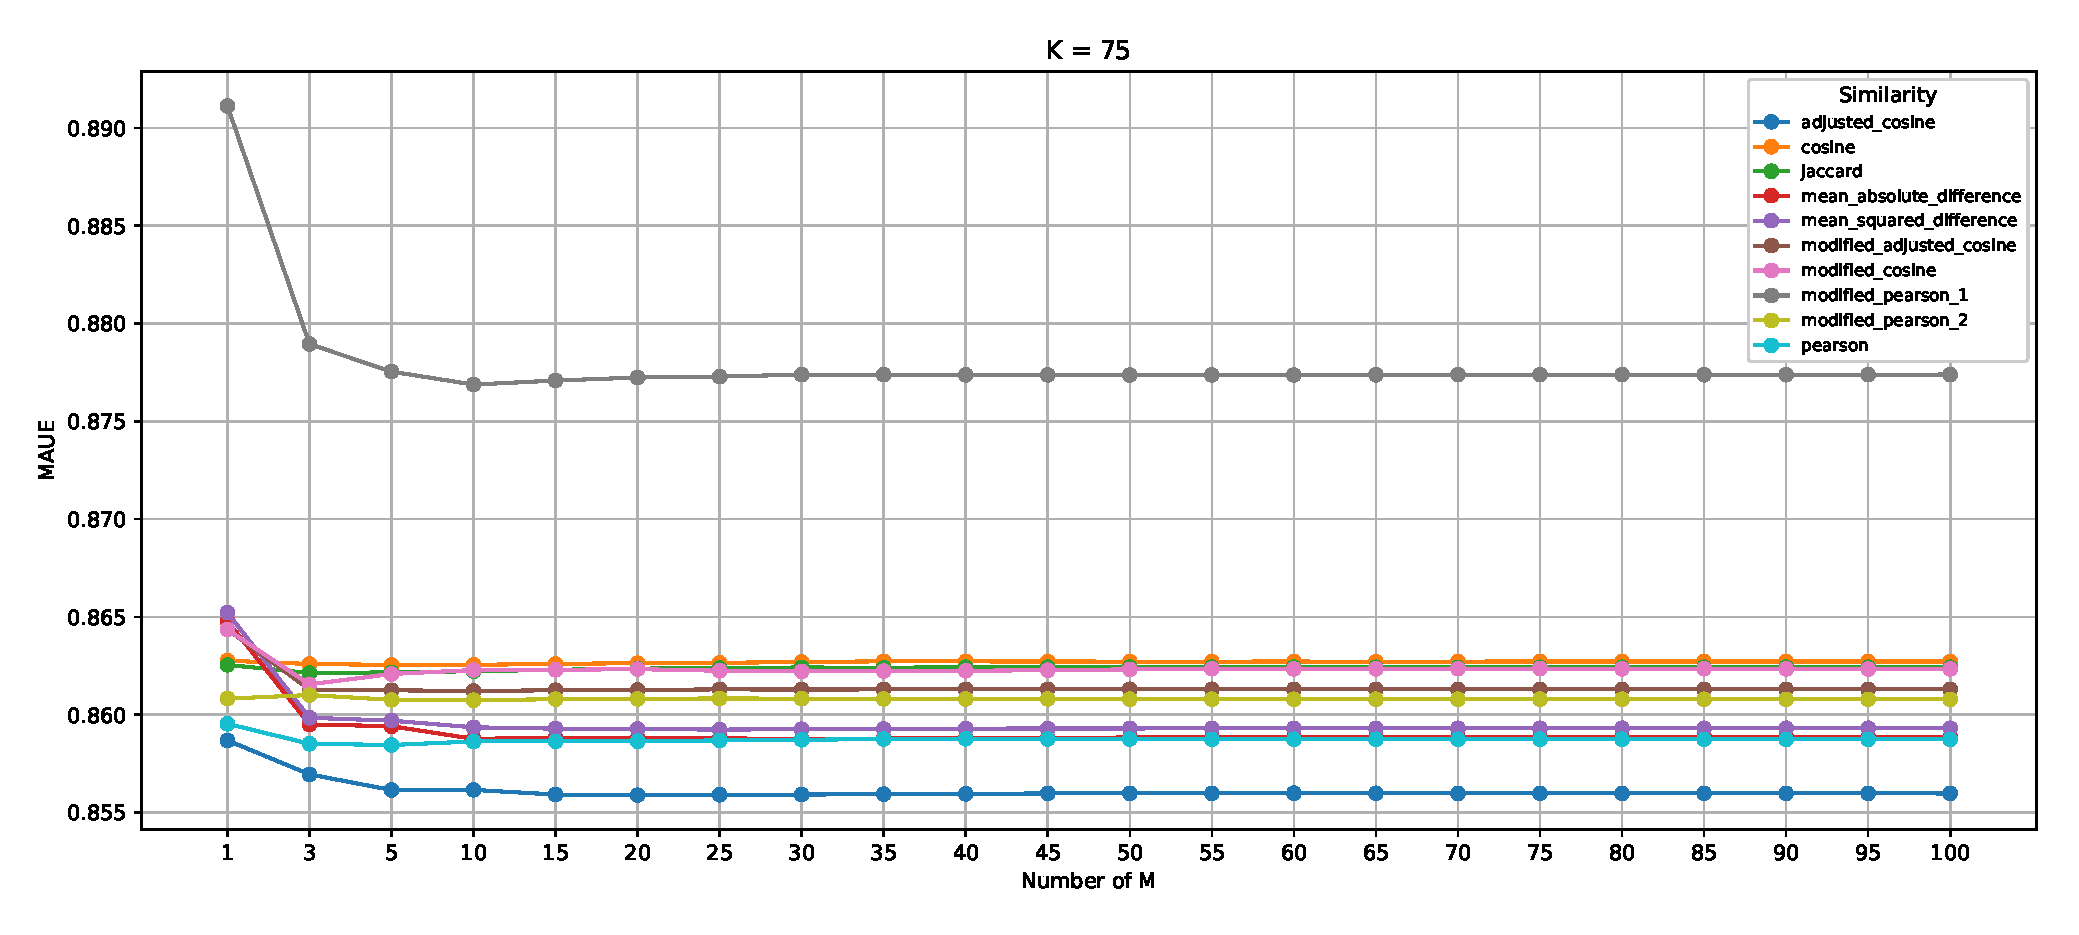
\includegraphics[width=1\textwidth,height=0.6\textheight]{evaluation_user_maue.eps}
    \end{figure}
    \centering
    \tiny
    Adjusted cosine at K=75 \& M=20, MAUE=0.8558869566
\end{columns}
\end{frame}
\begin{frame}[t]
    \frametitle{Item-based KNN and Total RMSE}
    \vspace{-0.7cm}
    \begin{columns}
        \column{0.5\textwidth}
        \centering
        \underline{\textbf{KNN}}
    \begin{figure}
    \centering
    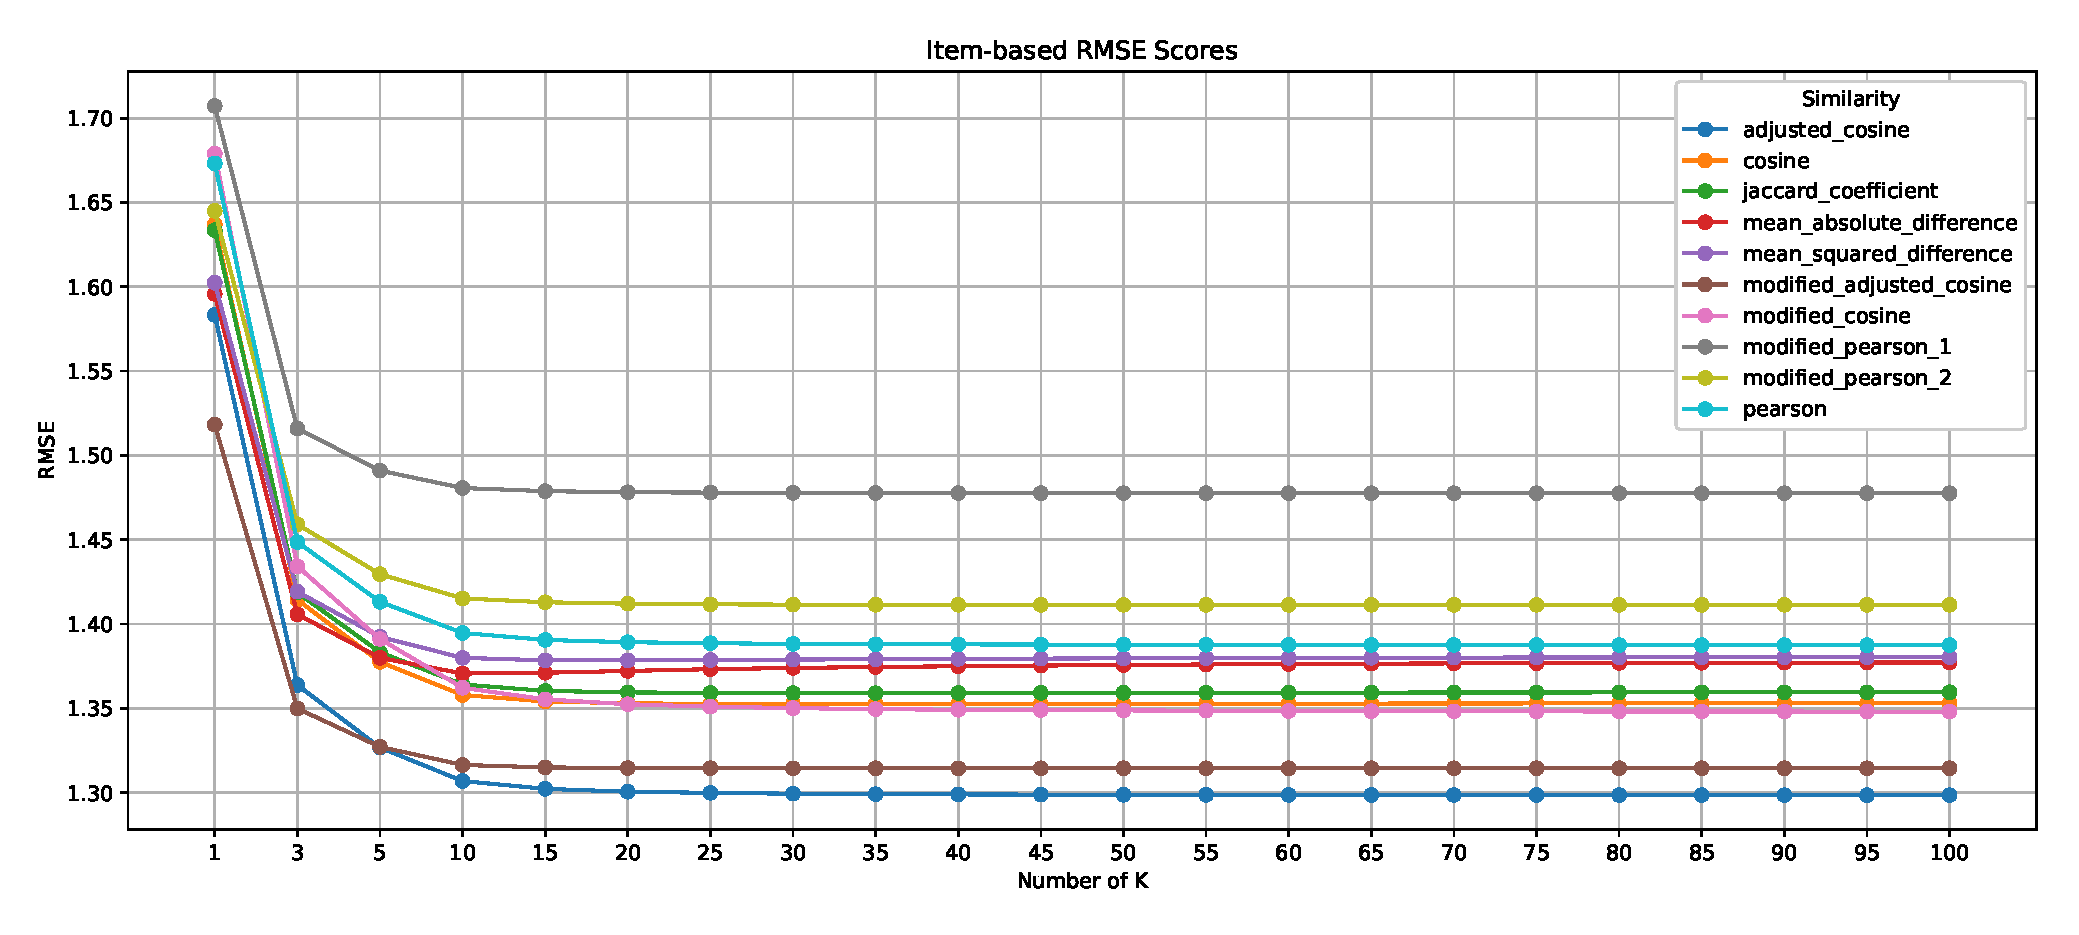
\includegraphics[width=1\textwidth,height=0.6\textheight]{Item_RMSE_KNN.eps}
    \end{figure}
    \centering
    \tiny
    Adjusted cosine at K=95, RMSE=1.2984970982
        \column{0.5\textwidth}
        \centering
        \underline{\textbf{Total}}
    \begin{figure}
    \centering
    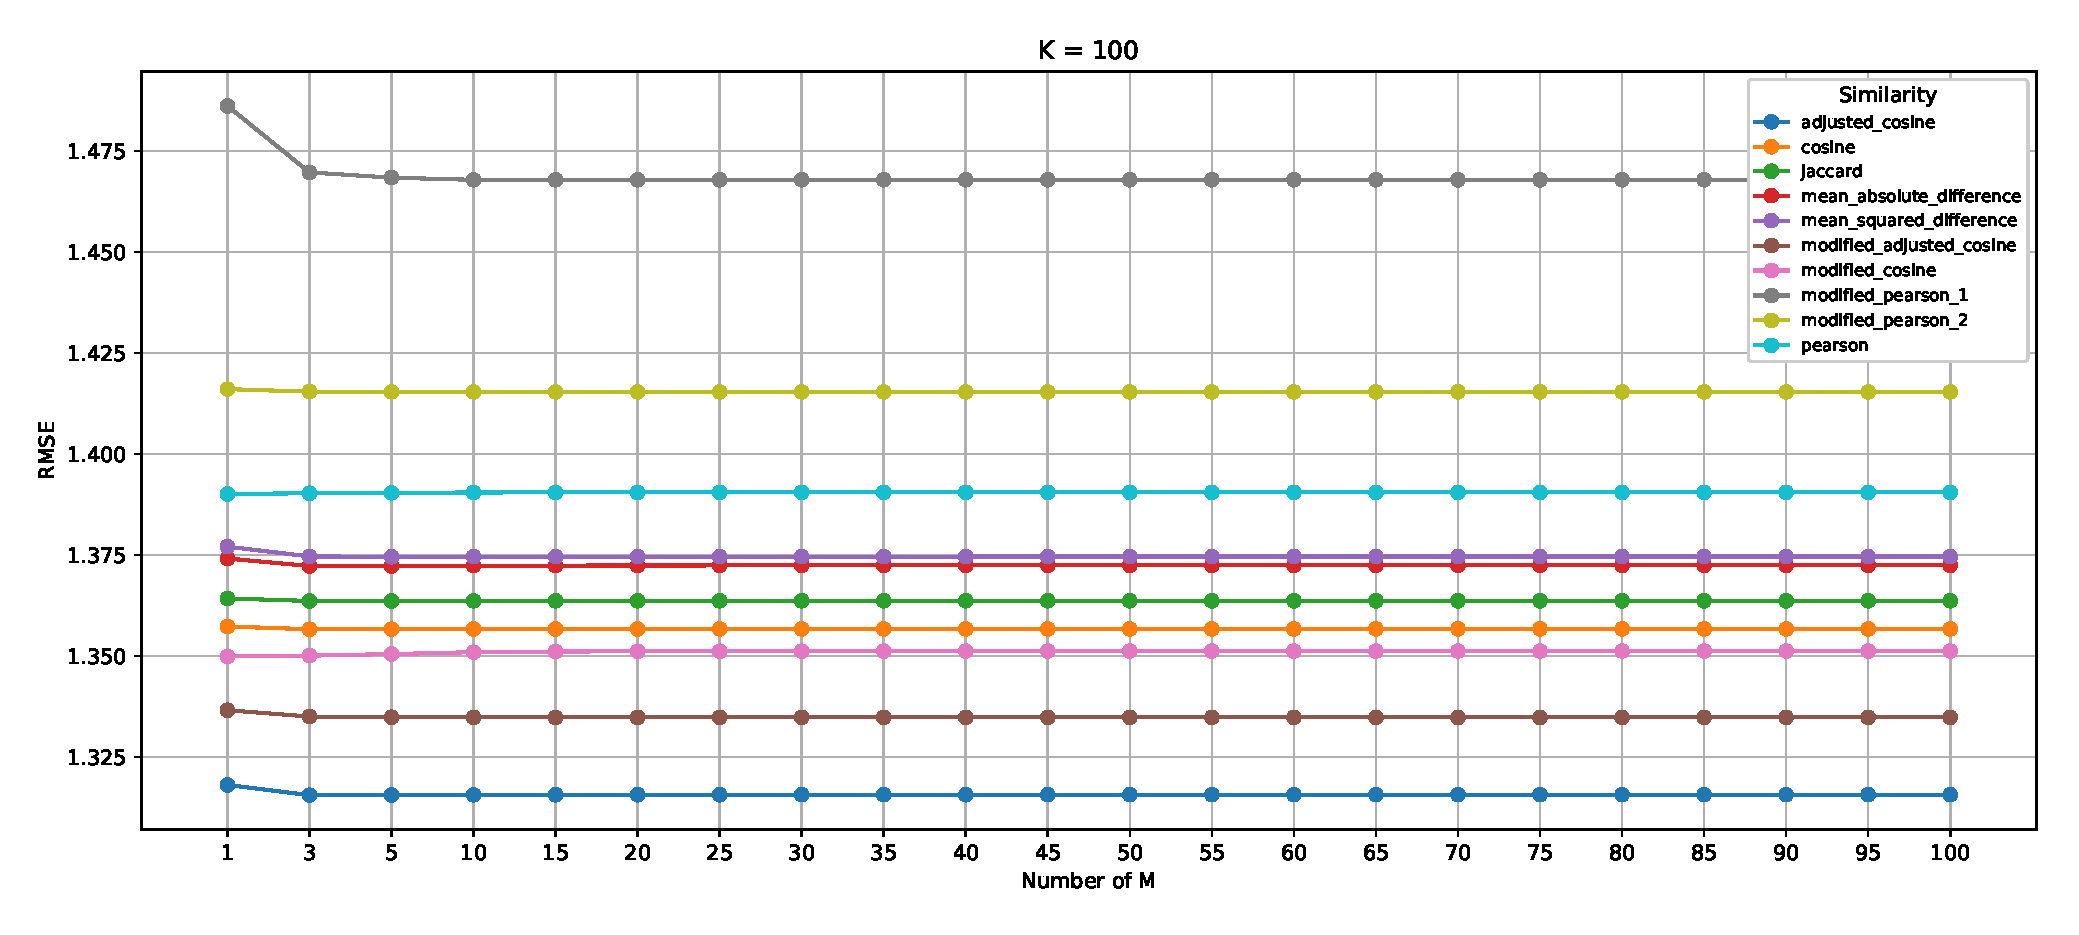
\includegraphics[width=1\textwidth,height=0.6\textheight]{evaluation_item_rmse.eps}
    \end{figure}
    \centering
    \tiny
    Adjusted cosine at K=100 \& M=3, RMSE=1.3155259043
\end{columns}
\end{frame}
\begin{frame}[t]
    \frametitle{Item-based KNN and Total MAE}
        \vspace{-0.7cm}
        \begin{columns}
            \column{0.5\textwidth}
            \centering
            \underline{\textbf{KNN}}
        \begin{figure}
        \centering
        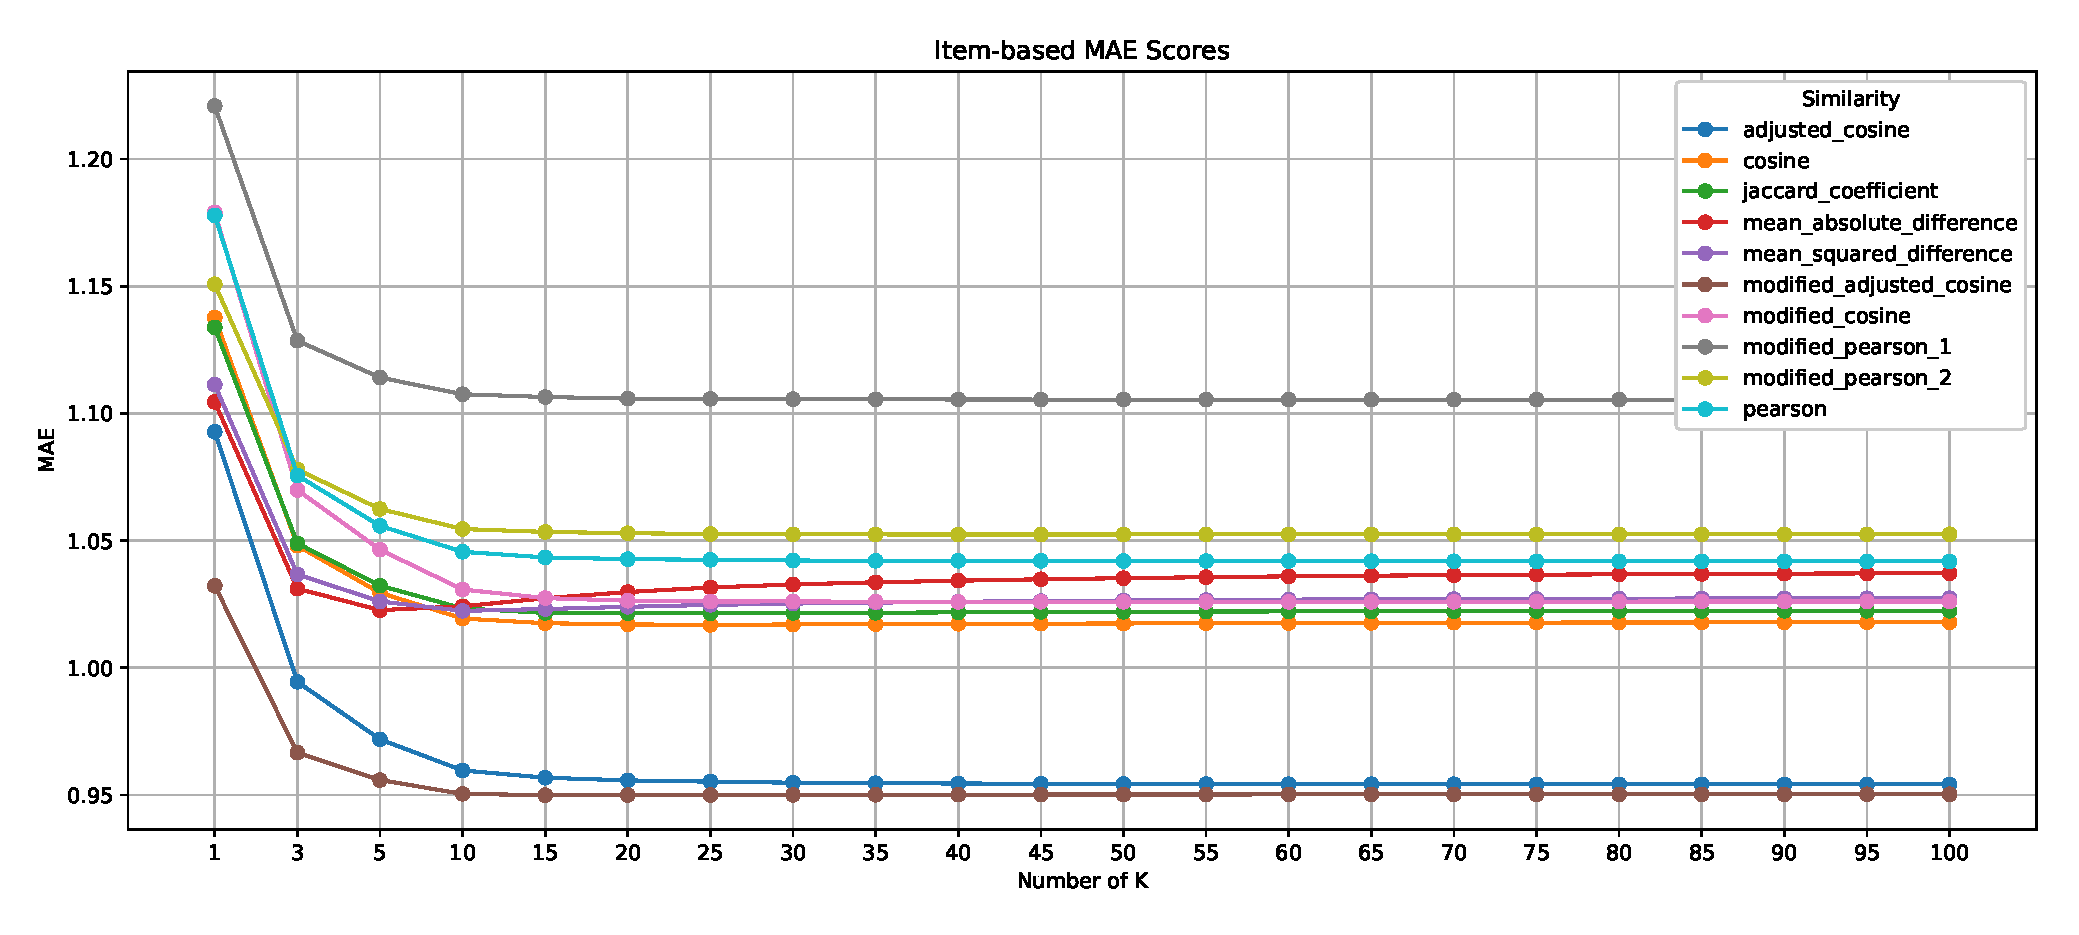
\includegraphics[width=1\textwidth,height=0.6\textheight]{Item_MAE_KNN.eps}
        \end{figure}
        \centering
        \tiny
        Modified adjusted cosine at K=15, MAE=0.9499219326
            \column{0.5\textwidth}
            \centering
            \underline{\textbf{Total}}
        \begin{figure}
        \centering
        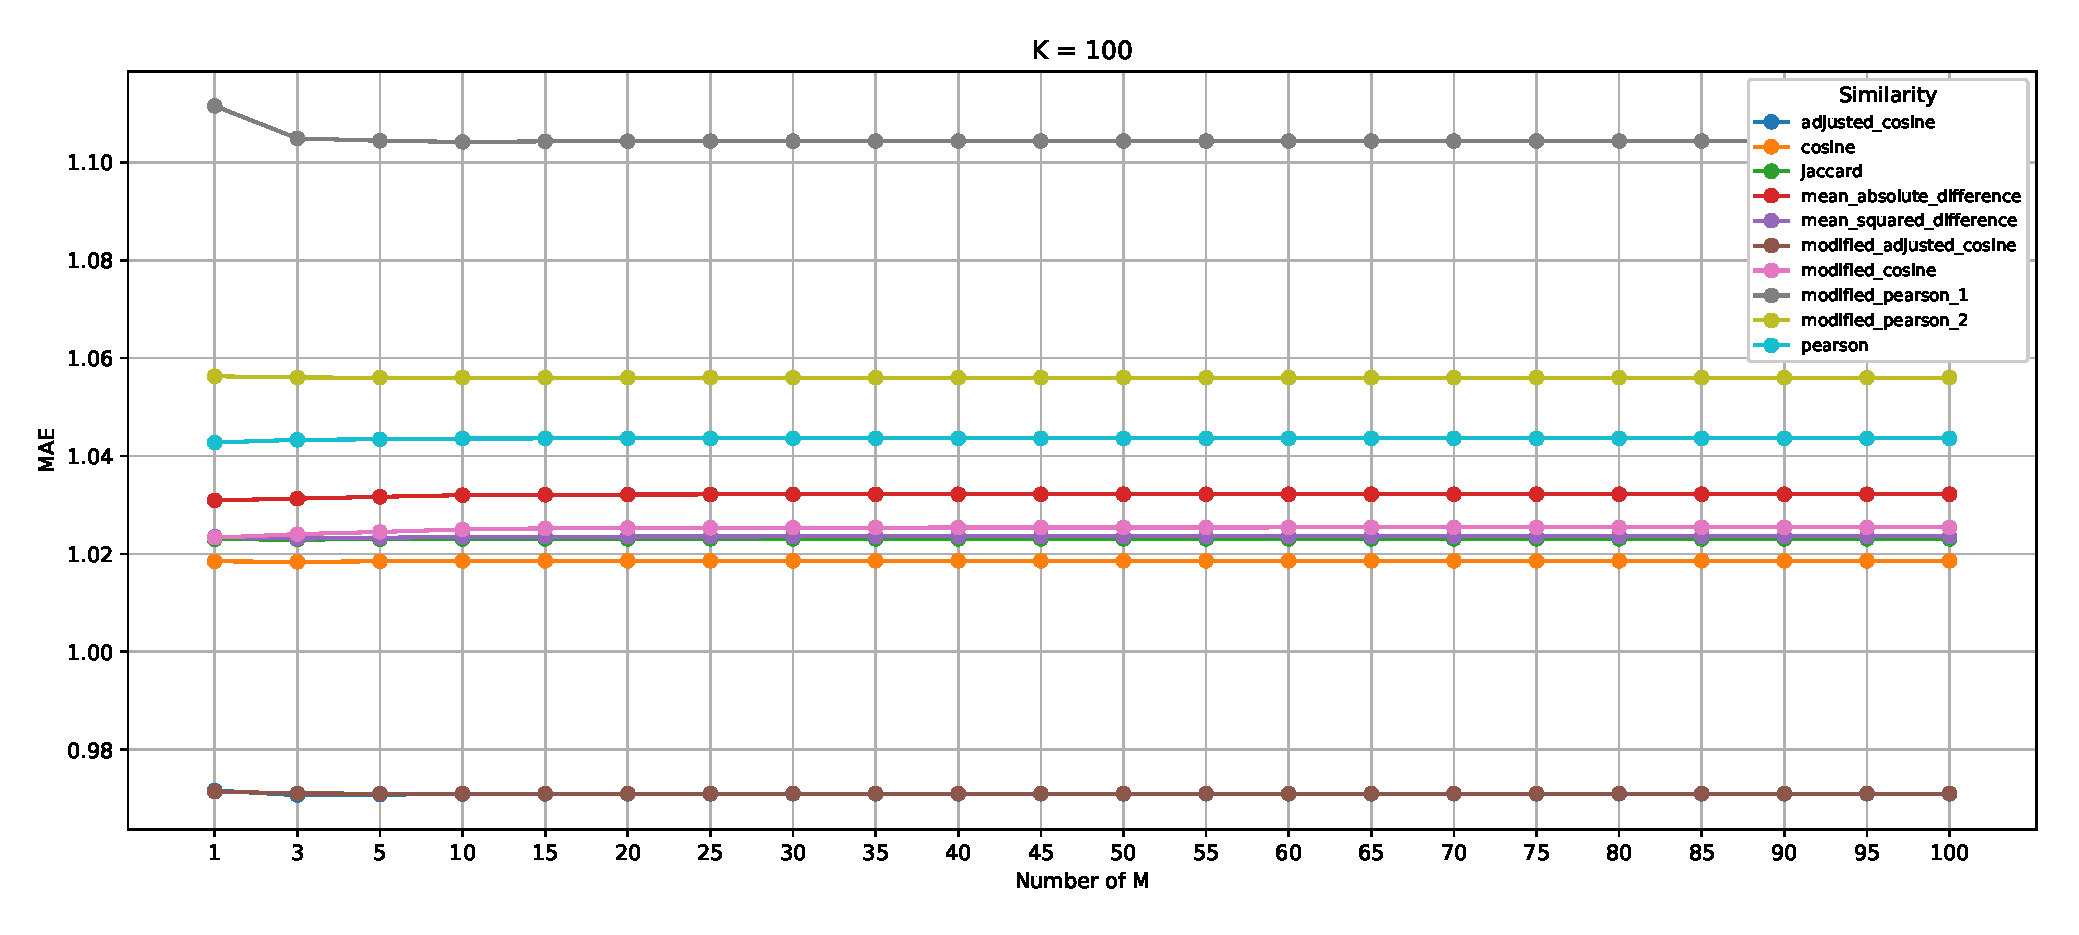
\includegraphics[width=1\textwidth,height=0.6\textheight]{evaluation_item_mae.eps}
        \end{figure}
        \centering
        \tiny
        Adjusted cosine at K=100 \& M=3, MAE=0.9707211649
    \end{columns}
\end{frame}
\begin{frame}[t]
    \frametitle{Item-based KNN and Recursive-KNN RMSUE}
    \vspace{-0.7cm}
    \begin{columns}
        \column{0.5\textwidth}
        \centering
        \underline{\textbf{KNN}}
    \begin{figure}
    \centering
    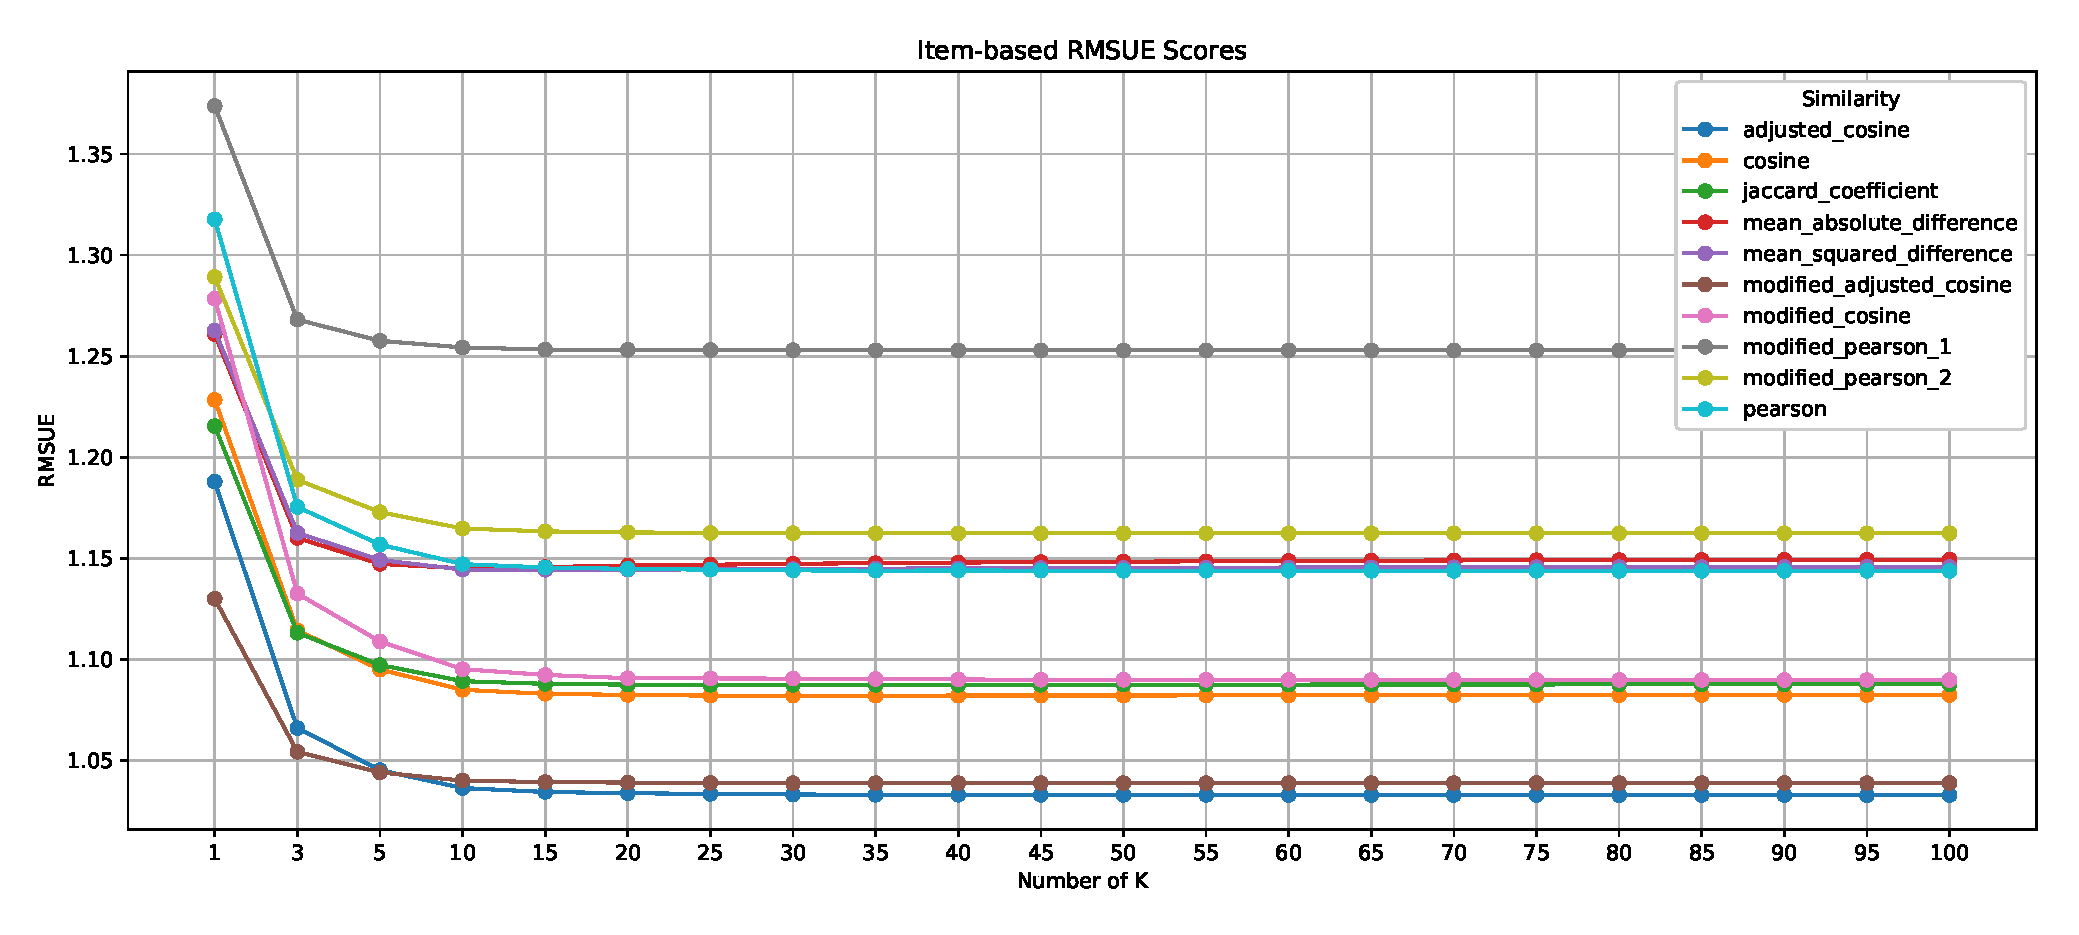
\includegraphics[width=1\textwidth,height=0.6\textheight]{Item_RMSUE_KNN.eps}
    \end{figure}
    \centering
    \tiny
    Adjusted cosine at K=100, RMSUE=1.0328968801
        \column{0.5\textwidth}
        \centering
        \underline{\textbf{Recursive-KNN}}
    \begin{figure}
    \centering
    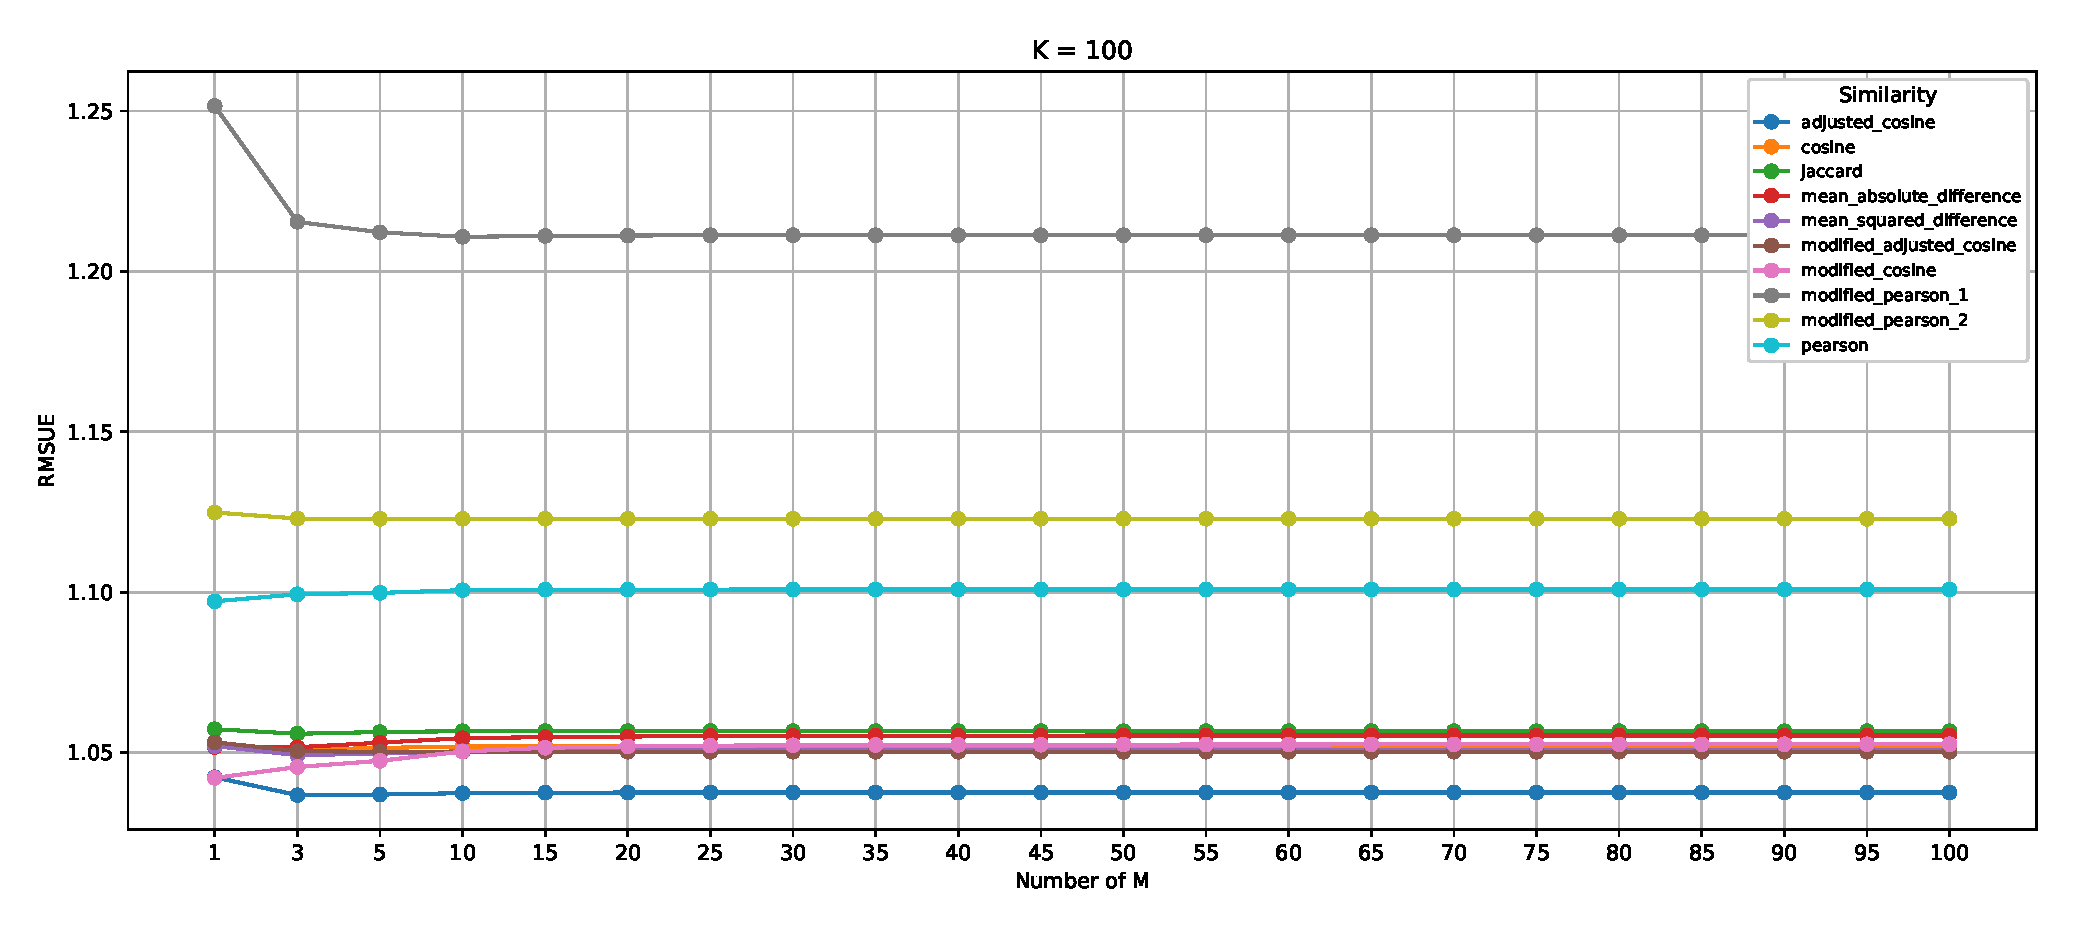
\includegraphics[width=1\textwidth,height=0.6\textheight]{evaluation_item_rmsue.eps}
    \end{figure}
    \centering
    \tiny
    Adjusted cosine at K=100 \& M=3, RMSUE=1.0367245756
\end{columns}
\end{frame}
\begin{frame}[t]
    \frametitle{Item-based KNN and Recursive-KNN MAUE}
    \vspace{-0.7cm}
    \begin{columns}
        \column{0.5\textwidth}
        \centering
        \underline{\textbf{KNN}}
    \begin{figure}
    \centering
    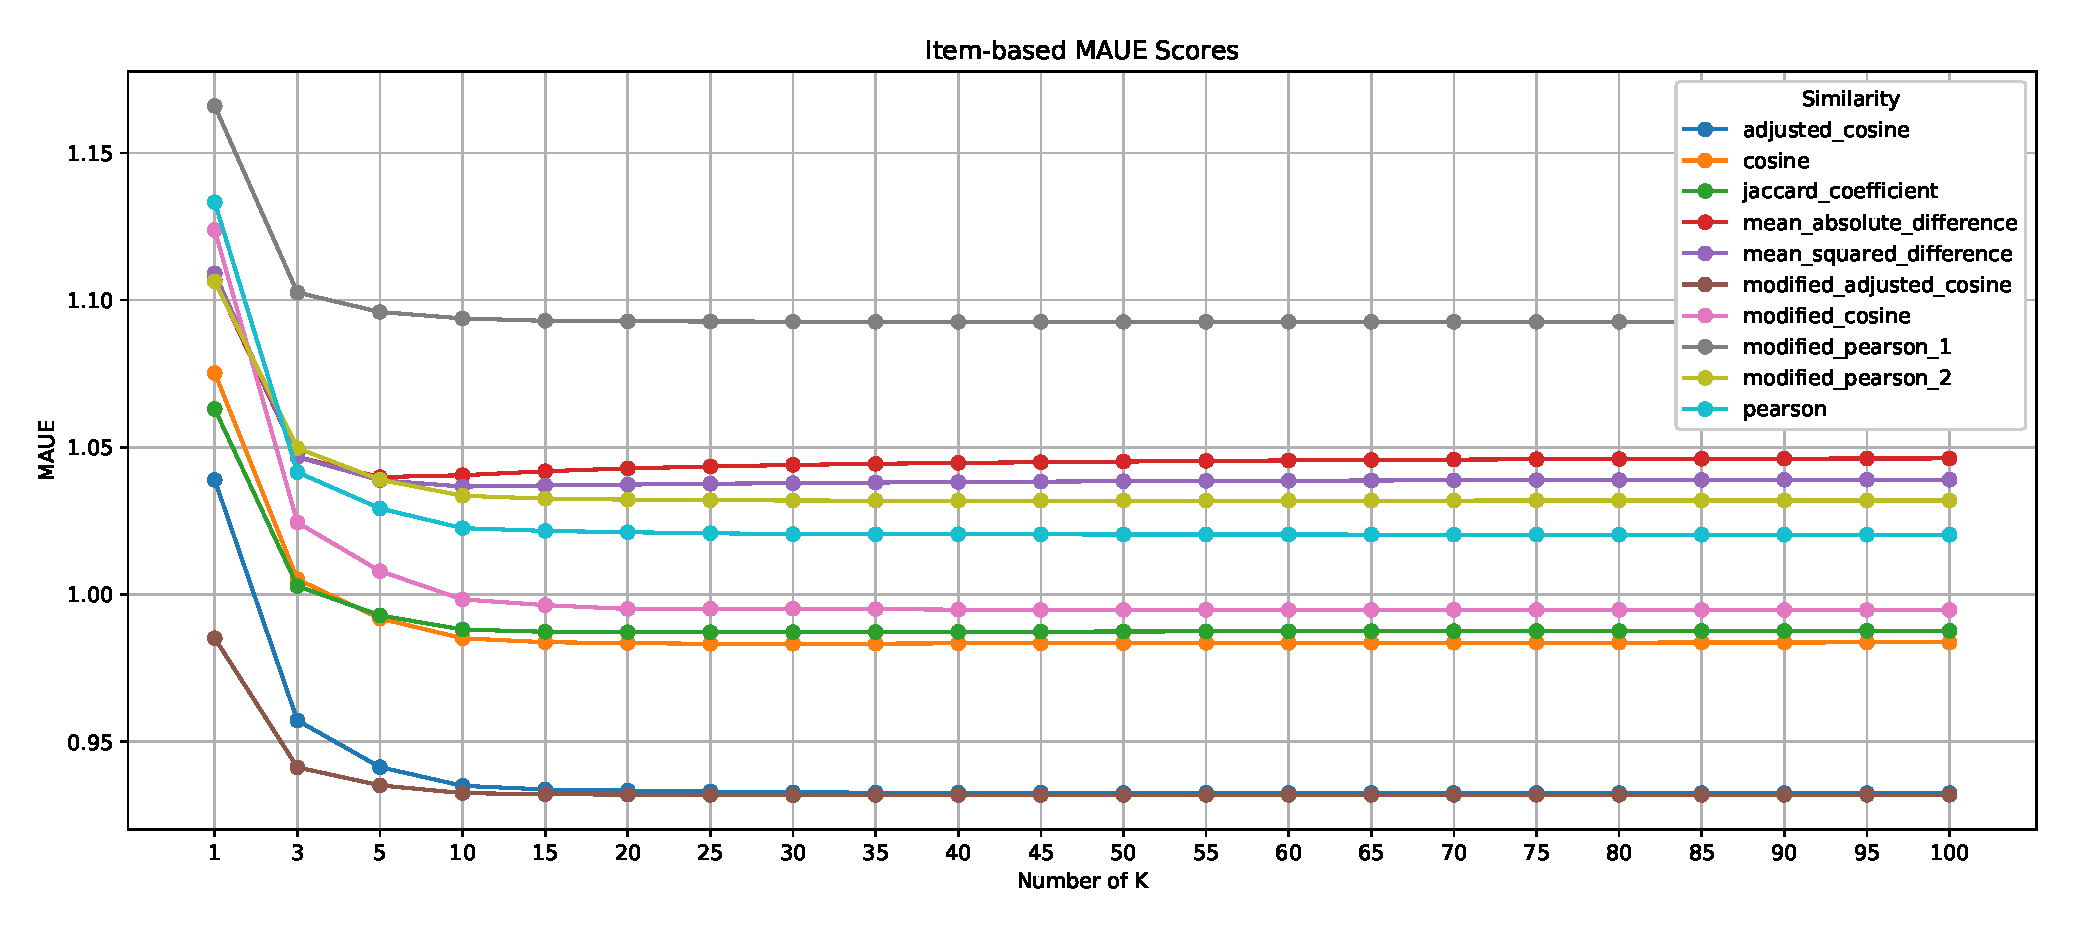
\includegraphics[width=1\textwidth,height=0.6\textheight]{Item_MAUE_KNN.eps}
    \end{figure}
    \centering
    \tiny
    Modified adjusted cosine at K=30, MAUE=0.9318609947
        \column{0.5\textwidth}
        \centering
        \underline{\textbf{Recursive-KNN}}
    \begin{figure}
    \centering
    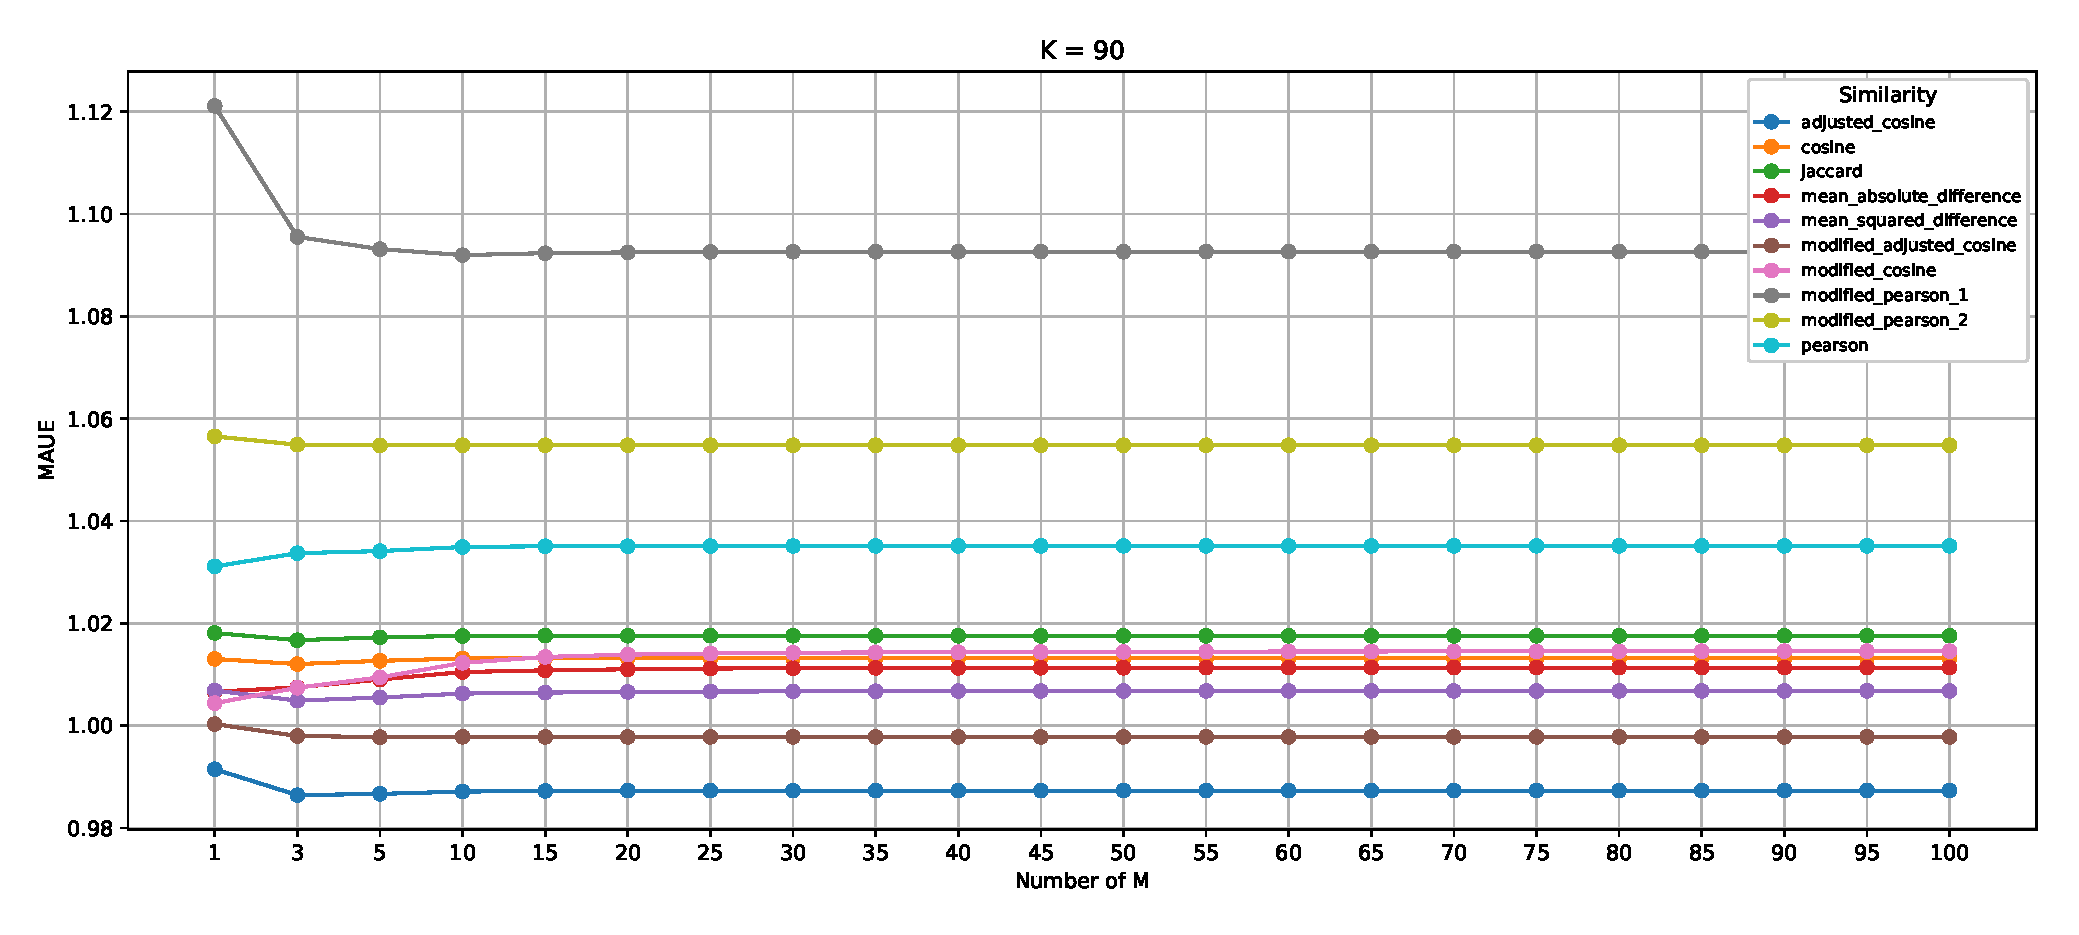
\includegraphics[width=1\textwidth,height=0.6\textheight]{evaluation_item_maue.eps}
    \end{figure}
    \centering
    \tiny
    Adjusted cosine at K=90 \& M=3, MAUE=0.9864005988
\end{columns}
\end{frame}

%---------------------------------------------------------------Conclusion----------------------------------------------------------------------------------------------------------
\section{Conclusion and Future Work}
\begin{frame}
    \frametitle{Conclusion}
    \begin{itemize}
        \item A novel recursive approach for Neighborhood-based CF
        \item 25\% increase in rating predictions
        \item Decent Results in User-based approach
    \end{itemize}
\end{frame}
\begin{frame}
    \frametitle{Future Work}
    \begin{itemize}
        \item Further use of similarity information
        \item Similarity re-computations including predictions
        \item Different prediction models
    \end{itemize}
\end{frame}
%-----------------------------------------------------------------Q & A-------------------------------------------------------------------------------------------------------------
\section{Q \& A}
\begin{frame}
    \frametitle{Q \& A}
    \centering
    \textbf{Any Questions?}
\end{frame}
\begin{frame}
    \centering
    \textbf{Thank You!}
\end{frame}
\end{document}
